\documentclass[11pt]{beamer}
\setbeamertemplate{navigation symbols}{}
 \setbeamercovered{transparent}
\usepackage{amsmath,amssymb,amsthm}
\usepackage{listings}
%\usetheme{Copenhagen}
\usetheme{Singapore}
%\usetheme{Madrid}
%\usetheme{Hannover}
%\usetheme{boxes}
%\usetheme{Boadilla}
%\usepackage[margin=1in]{geometry}
\usefonttheme[onlymath]{serif}
\usecolortheme{beaver}
\usepackage{textpos}
\usepackage{fancyvrb}
%\usepackage{listings}
\usepackage{xcolor}
\usepackage{multicol}
\usepackage{lipsum}
\usepackage{fancyvrb}
\usepackage{color}

\parskip 1ex

% ################### CODE LISTINGS ############################
%\usepackage{listings}     
\usepackage{lstautogobble}  % Fix relative indenting
%\usepackage{color}          % Code coloring
\usepackage{zi4}            % Nice font

\definecolor{bluekeywords}{rgb}{0.13, 0.13, 1}
\definecolor{greencomments}{rgb}{0, 0.5, 0}
\definecolor{redstrings}{rgb}{0.9, 0, 0}
\definecolor{graynumbers}{rgb}{0.5, 0.5, 0.5}

\lstset{
    language=bash,
    autogobble,
    columns=fullflexible,
    showspaces=false,
    showtabs=false,
    breaklines=true,
    showstringspaces=false,
    breakatwhitespace=true,
    escapeinside={(*@}{@*)},
    commentstyle=\color{greencomments},
    %keywordstyle=\color{bluekeywords},
    stringstyle=\color{redstrings},
    numberstyle=\color{graynumbers},
    basicstyle=\ttfamily\footnotesize,
    framesep=12pt,
    xleftmargin=12pt,
    tabsize=4,
    captionpos=b
    }

\newcommand\tab[1][1cm]{\hspace*{#1}}
\newcommand{\light}[1]{\textcolor{lightgray}{#1}}
    
\def\signed #1{{\leavevmode\unskip\nobreak\hfil\penalty50\hskip2em
  \hbox{}\nobreak\hfil(#1)%
  \parfillskip=0pt \finalhyphendemerits=0 \endgraf}}

\newsavebox\mybox
\newenvironment{aquote}[1]
  {\savebox\mybox{#1}\begin{quote}}
  {\signed{\usebox\mybox}\end{quote}}
  
% items enclosed in square brackets are optional; explanation below
\title{Version Control with Git}
\date{}

\begin{document}

% --- Title page ---
\begin{frame}[plain]
  \titlepage
\end{frame}

\logo{%
  
\includegraphics[width=1cm,height=1cm,keepaspectratio]{nasa-ball.png}%
  \hspace{\dimexpr\paperwidth-2cm-5pt}%
  
\includegraphics[width=1cm,height=1cm,keepaspectratio]{ssai-logo.png}%
}


% Tutorial is for 
% People that never used Git
% People that have used other VCSs
% People that have only used Git GUI tools

% One objective is to attempt to convince you that you need to use version control for your software projects
% give you some resources to learn more
% show you some examples of successful software
% hopefully show you something you haven't seen before

% --- Slide

\begin{frame}[fragile]
\frametitle{What is version control?}

% As scientists we want
%%  reproducible research
%%  fast and efficient research

\begin{figure}[htp]
 \centering
 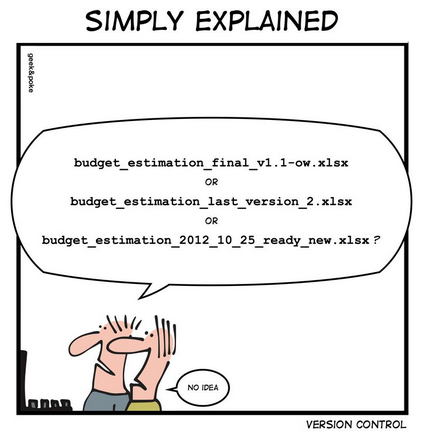
\includegraphics[scale=0.5]{version-control-comic.png}
\end{figure}

\end{frame}



% --- Slide

\begin{frame}[fragile]
\frametitle{What is version control?}

% Also called "source code control," "revision control," "source code versioning"

 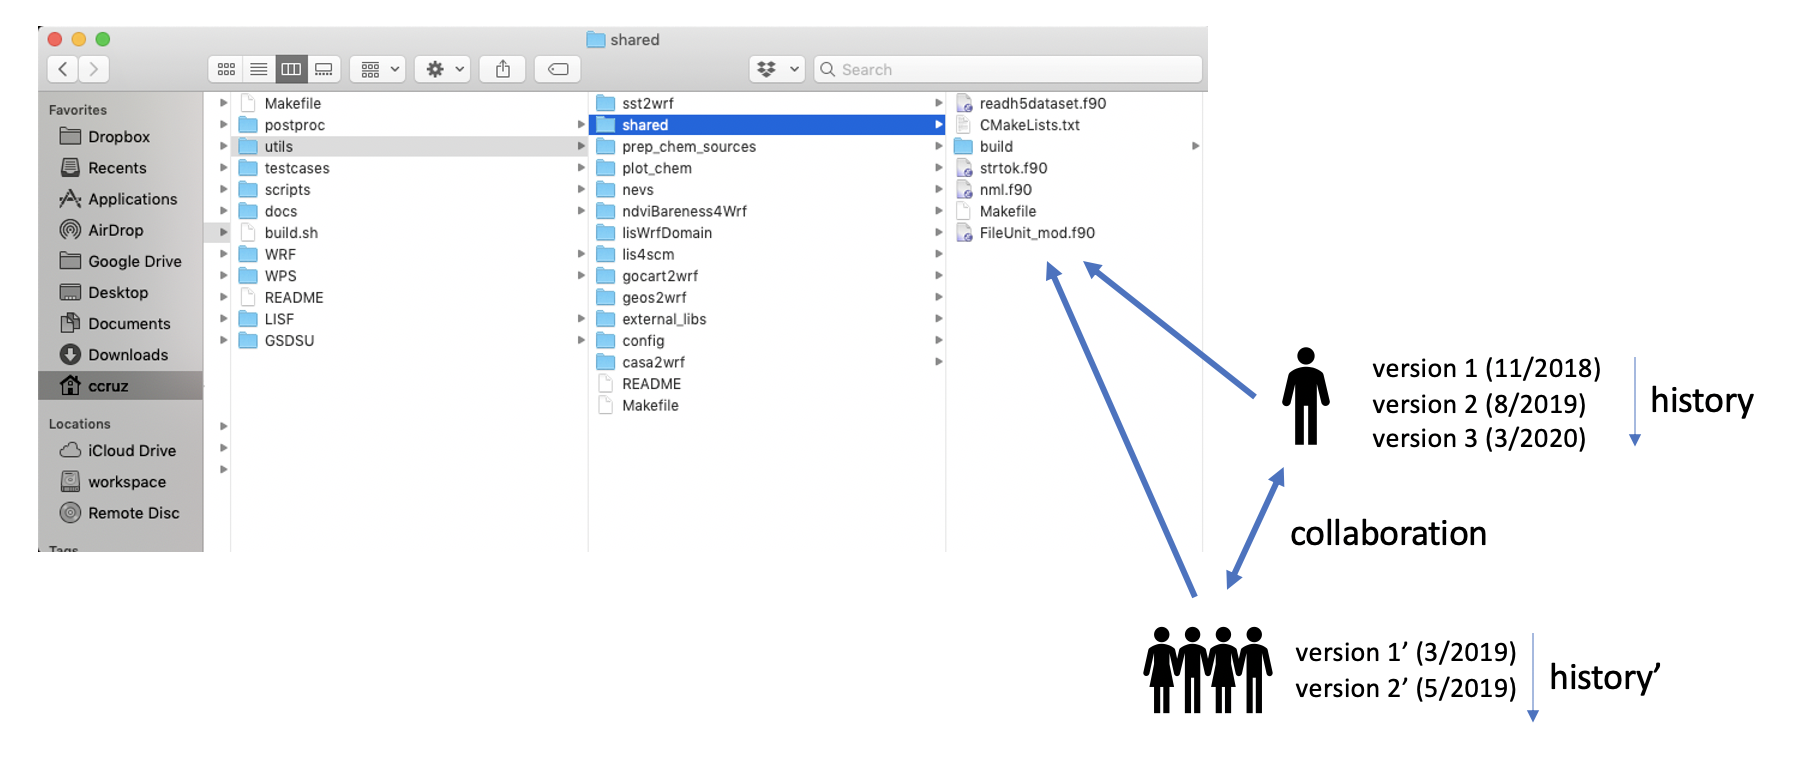
\includegraphics[scale=0.35]{what_is_a_vcs.png}


%A version control is a means of managing this process in a reliable and efficient way.}

% Also called "source code control," "revision control," "source code versioning"



\end{frame}


% Why do we care?

% Has been used by software developers for decades
% Source code lives in one or more repositories (repos) available to team members/contributors.
% A repo is a computational scientist?s laboratory notebook.
% Establishes a common context for code contributions and the exchange of ideas
% Establishes a chronological sequence of events
% Serves as "ground truth" for a software project
% Results from uncontrolled code are not \emph{reproducible}.


% --- Slide


%Advantages of using version control}\\
% A repo can tell you exactly what version you are looking at (with a unique identifier).
% Everyone can agree on whether they are looking at the same thing.
% If there are conflicts, your version control system will tell you, and \emph{you will need to resolve them}.


% What if I'm developing software by myself?
%% Version control offers you the same advantages/ legitimacy of a laboratory notebook
%% If you're developing your software on more than one machine, you still need to keep it consistent across these machines.
%% If you want to collaborate with someone congratulations! You're now in the same boat as software teams.

% --- Slide

\begin{frame}[fragile]
\frametitle{Centralized version control systems}

\centering
\footnotesize{In a central VCS there is \textbf{one} repository containing the master version (the "trunk") of the source code.}
\begin{figure}[htp]
 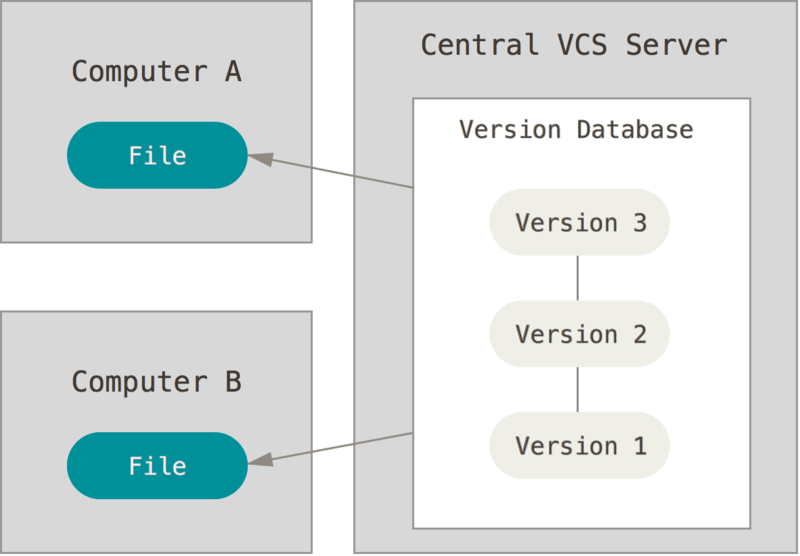
\includegraphics[scale=0.25]{centralized.png}
\end{figure}
 \tiny{Image source: \url{https://git-scm.com}}

\centering
\footnotesize{Example: SCCS, RCS, CVS, SVN}\\

%Most centralized systems (SCCS, RCS, CVS, SVN) don't allow the creation of separate development branches.


% Everyone syncs with this repository, checks out files, changes them, and commits these changes.
%% People must cooperate to make sure their changes don't conflict with each other.
%% Simple, but limited.

\end{frame}


% --- Slide

\begin{frame}[fragile]
\frametitle{Distributed version control systems}

\centering
\begin{figure}[htp]
 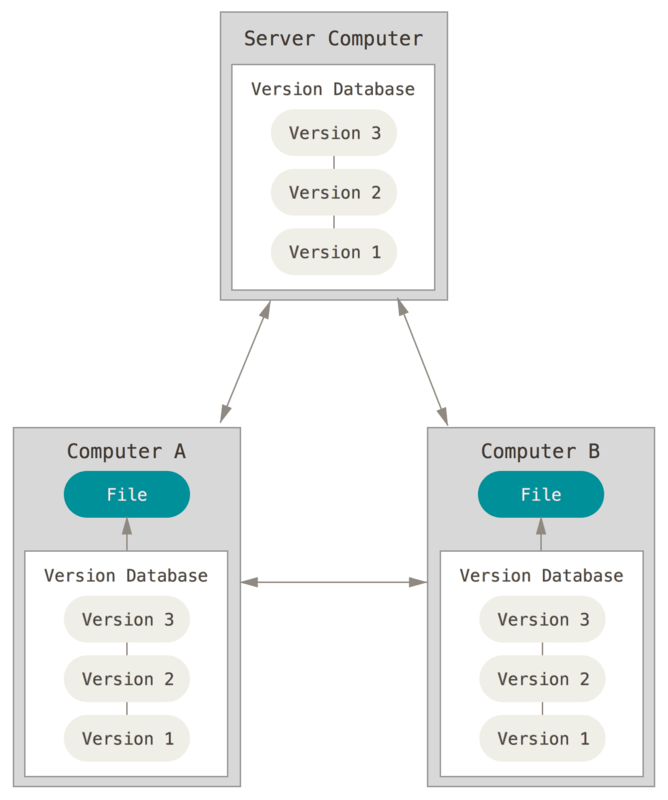
\includegraphics[scale=0.22]{distributed.png}
\end{figure}
 \tiny{Image source: \url{https://git-scm.com}}

\centering
\footnotesize{Example: Git, Mercurial}\\
\end{frame}



% --- Slide

\begin{frame}[fragile]
\frametitle{The Git concept}

\begin{figure}[htp]
 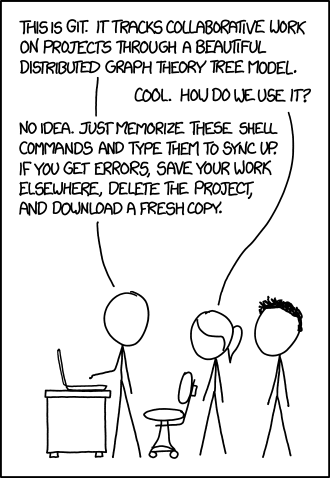
\includegraphics[scale=0.35]{what-is-git.png}
 
\end{figure}

%\begin{verbatim}
%Git is a free and open source distributed version control 
%system designed to handle everything from small to very
%large projects with speed and efficiency.
%\end{verbatim}
%\vspace{10px}
%\footnotesize{
%\textcolor{white}{Caveats:\\
%\quad Git is difficult to learn without putting in some time.\\
%\quad It's difficult to understand how Git works without knowing the underlying concepts.\\
%}}
% most commonly used VCS
% Linus Torvalds

\end{frame}


% --- Slide

\begin{frame}[fragile]
\frametitle{The Git Model}

\begin{figure}[htp]
 \centering
 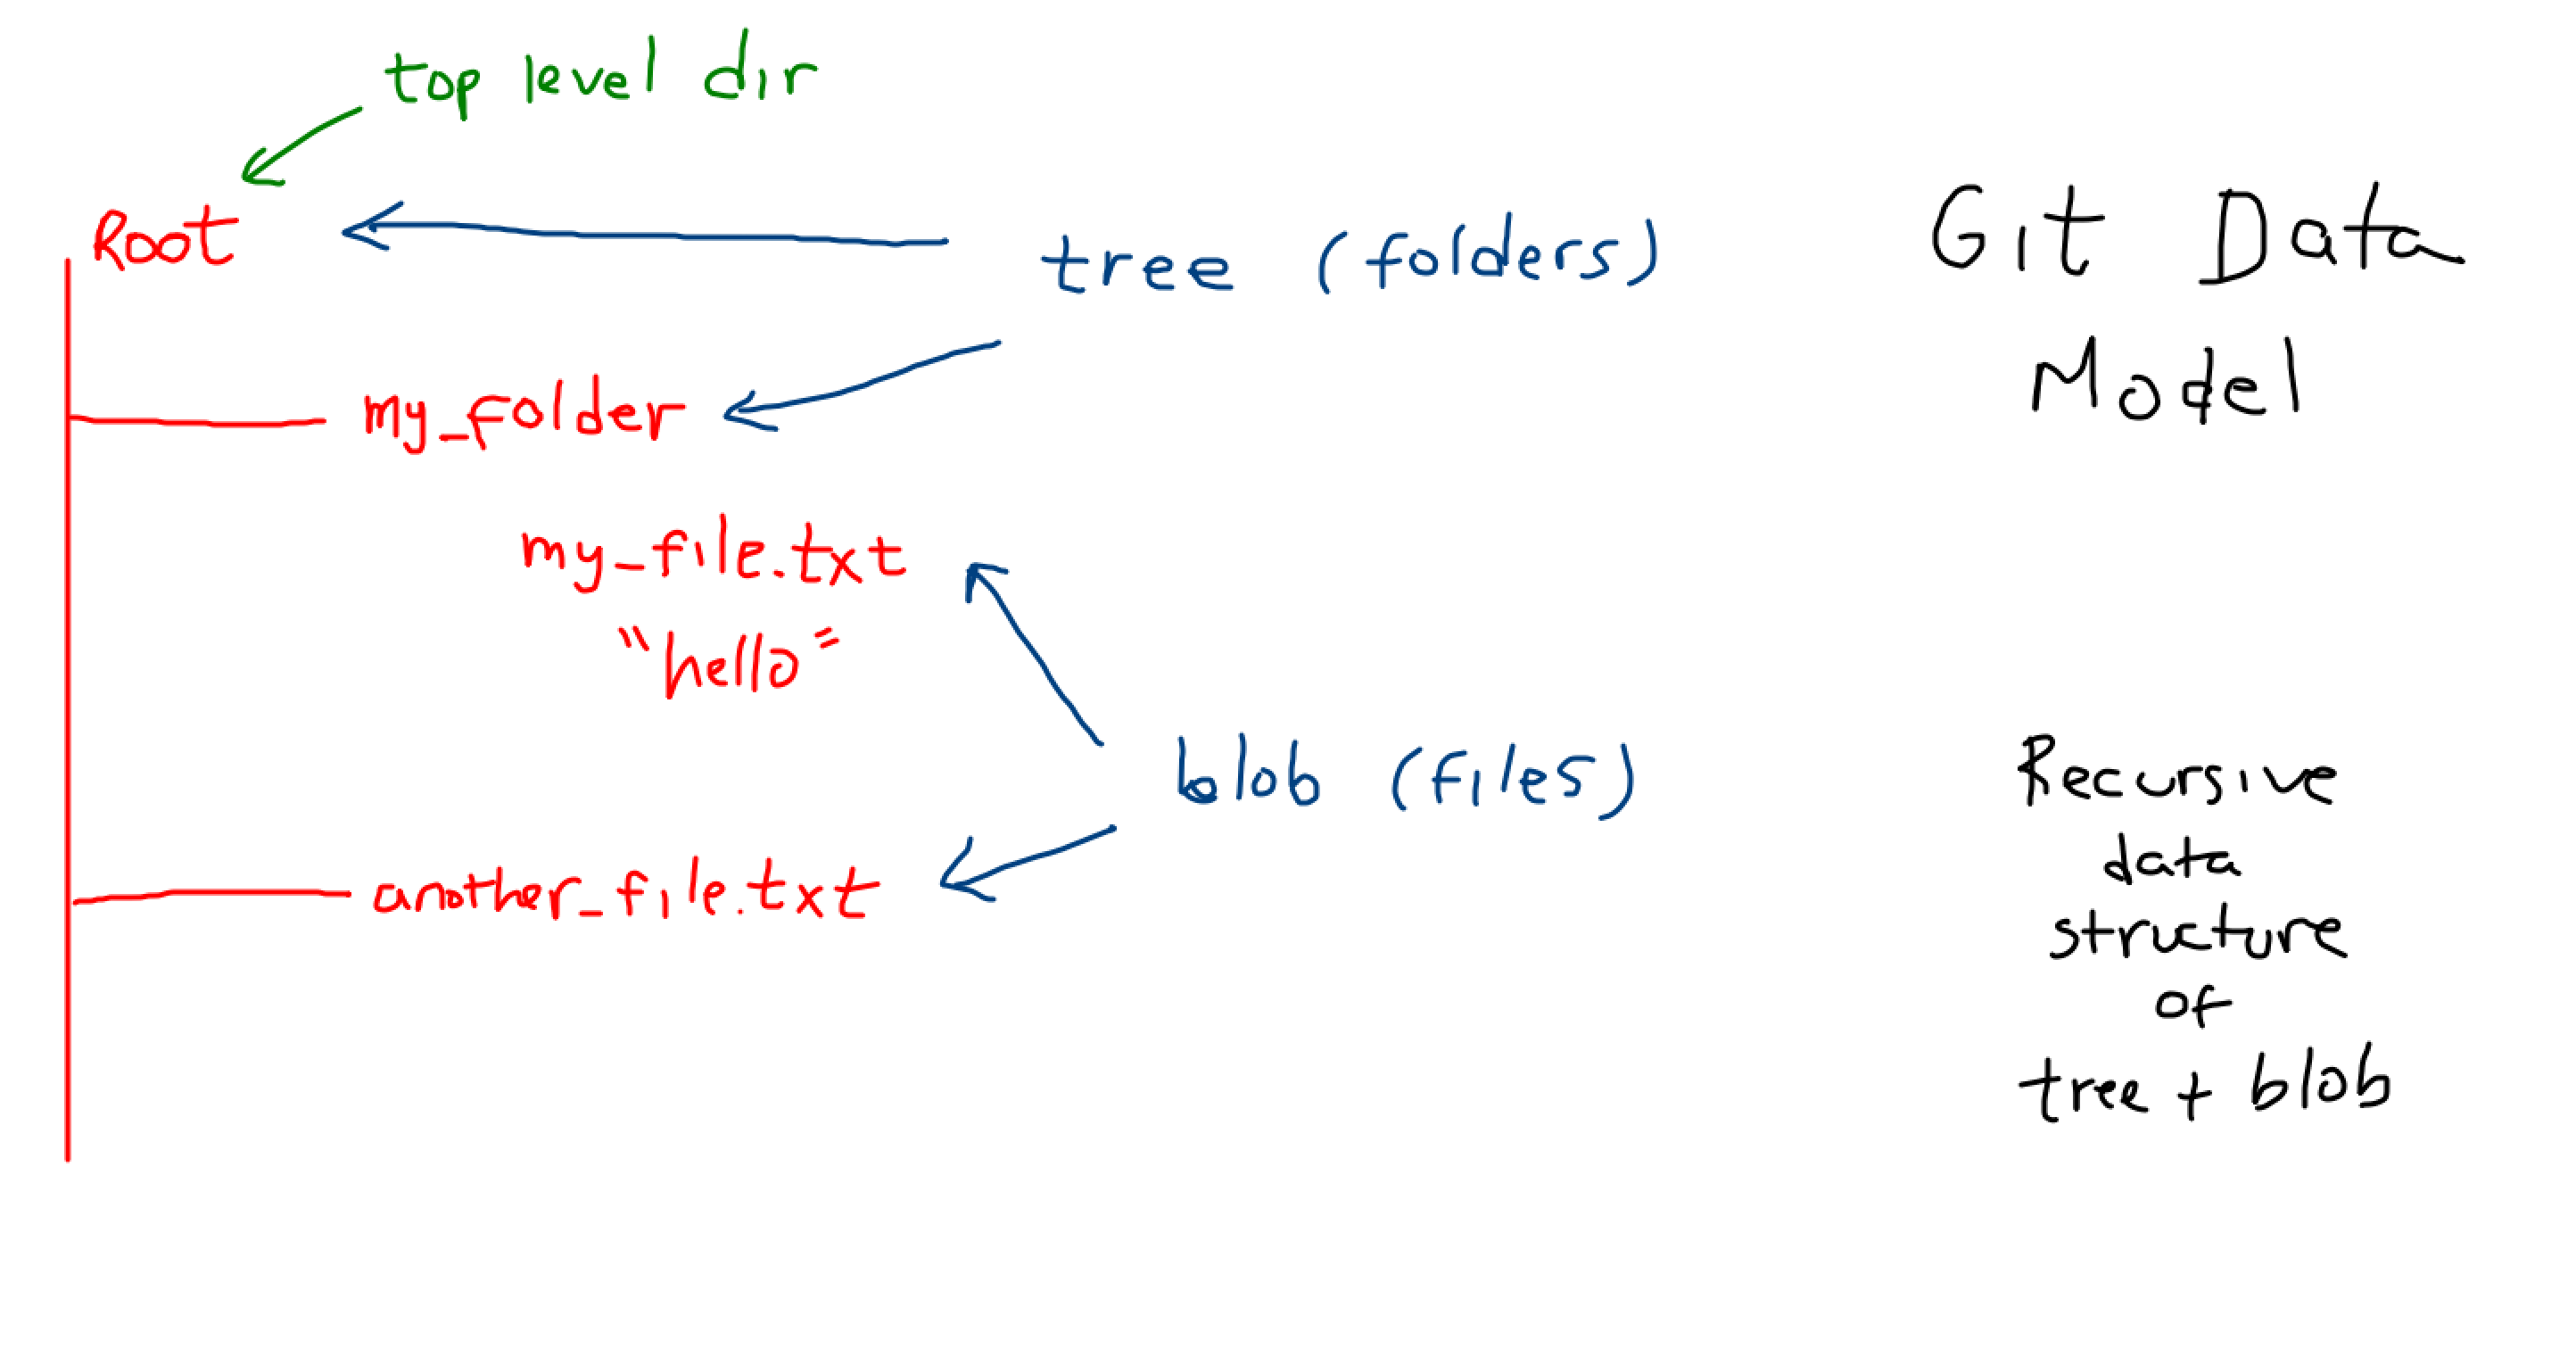
\includegraphics[scale=0.2]{git_model1.png}
\end{figure}

\end{frame}



% --- Slide

\begin{frame}[fragile]
\frametitle{The Git Model}

\begin{figure}[htp]
 \centering
 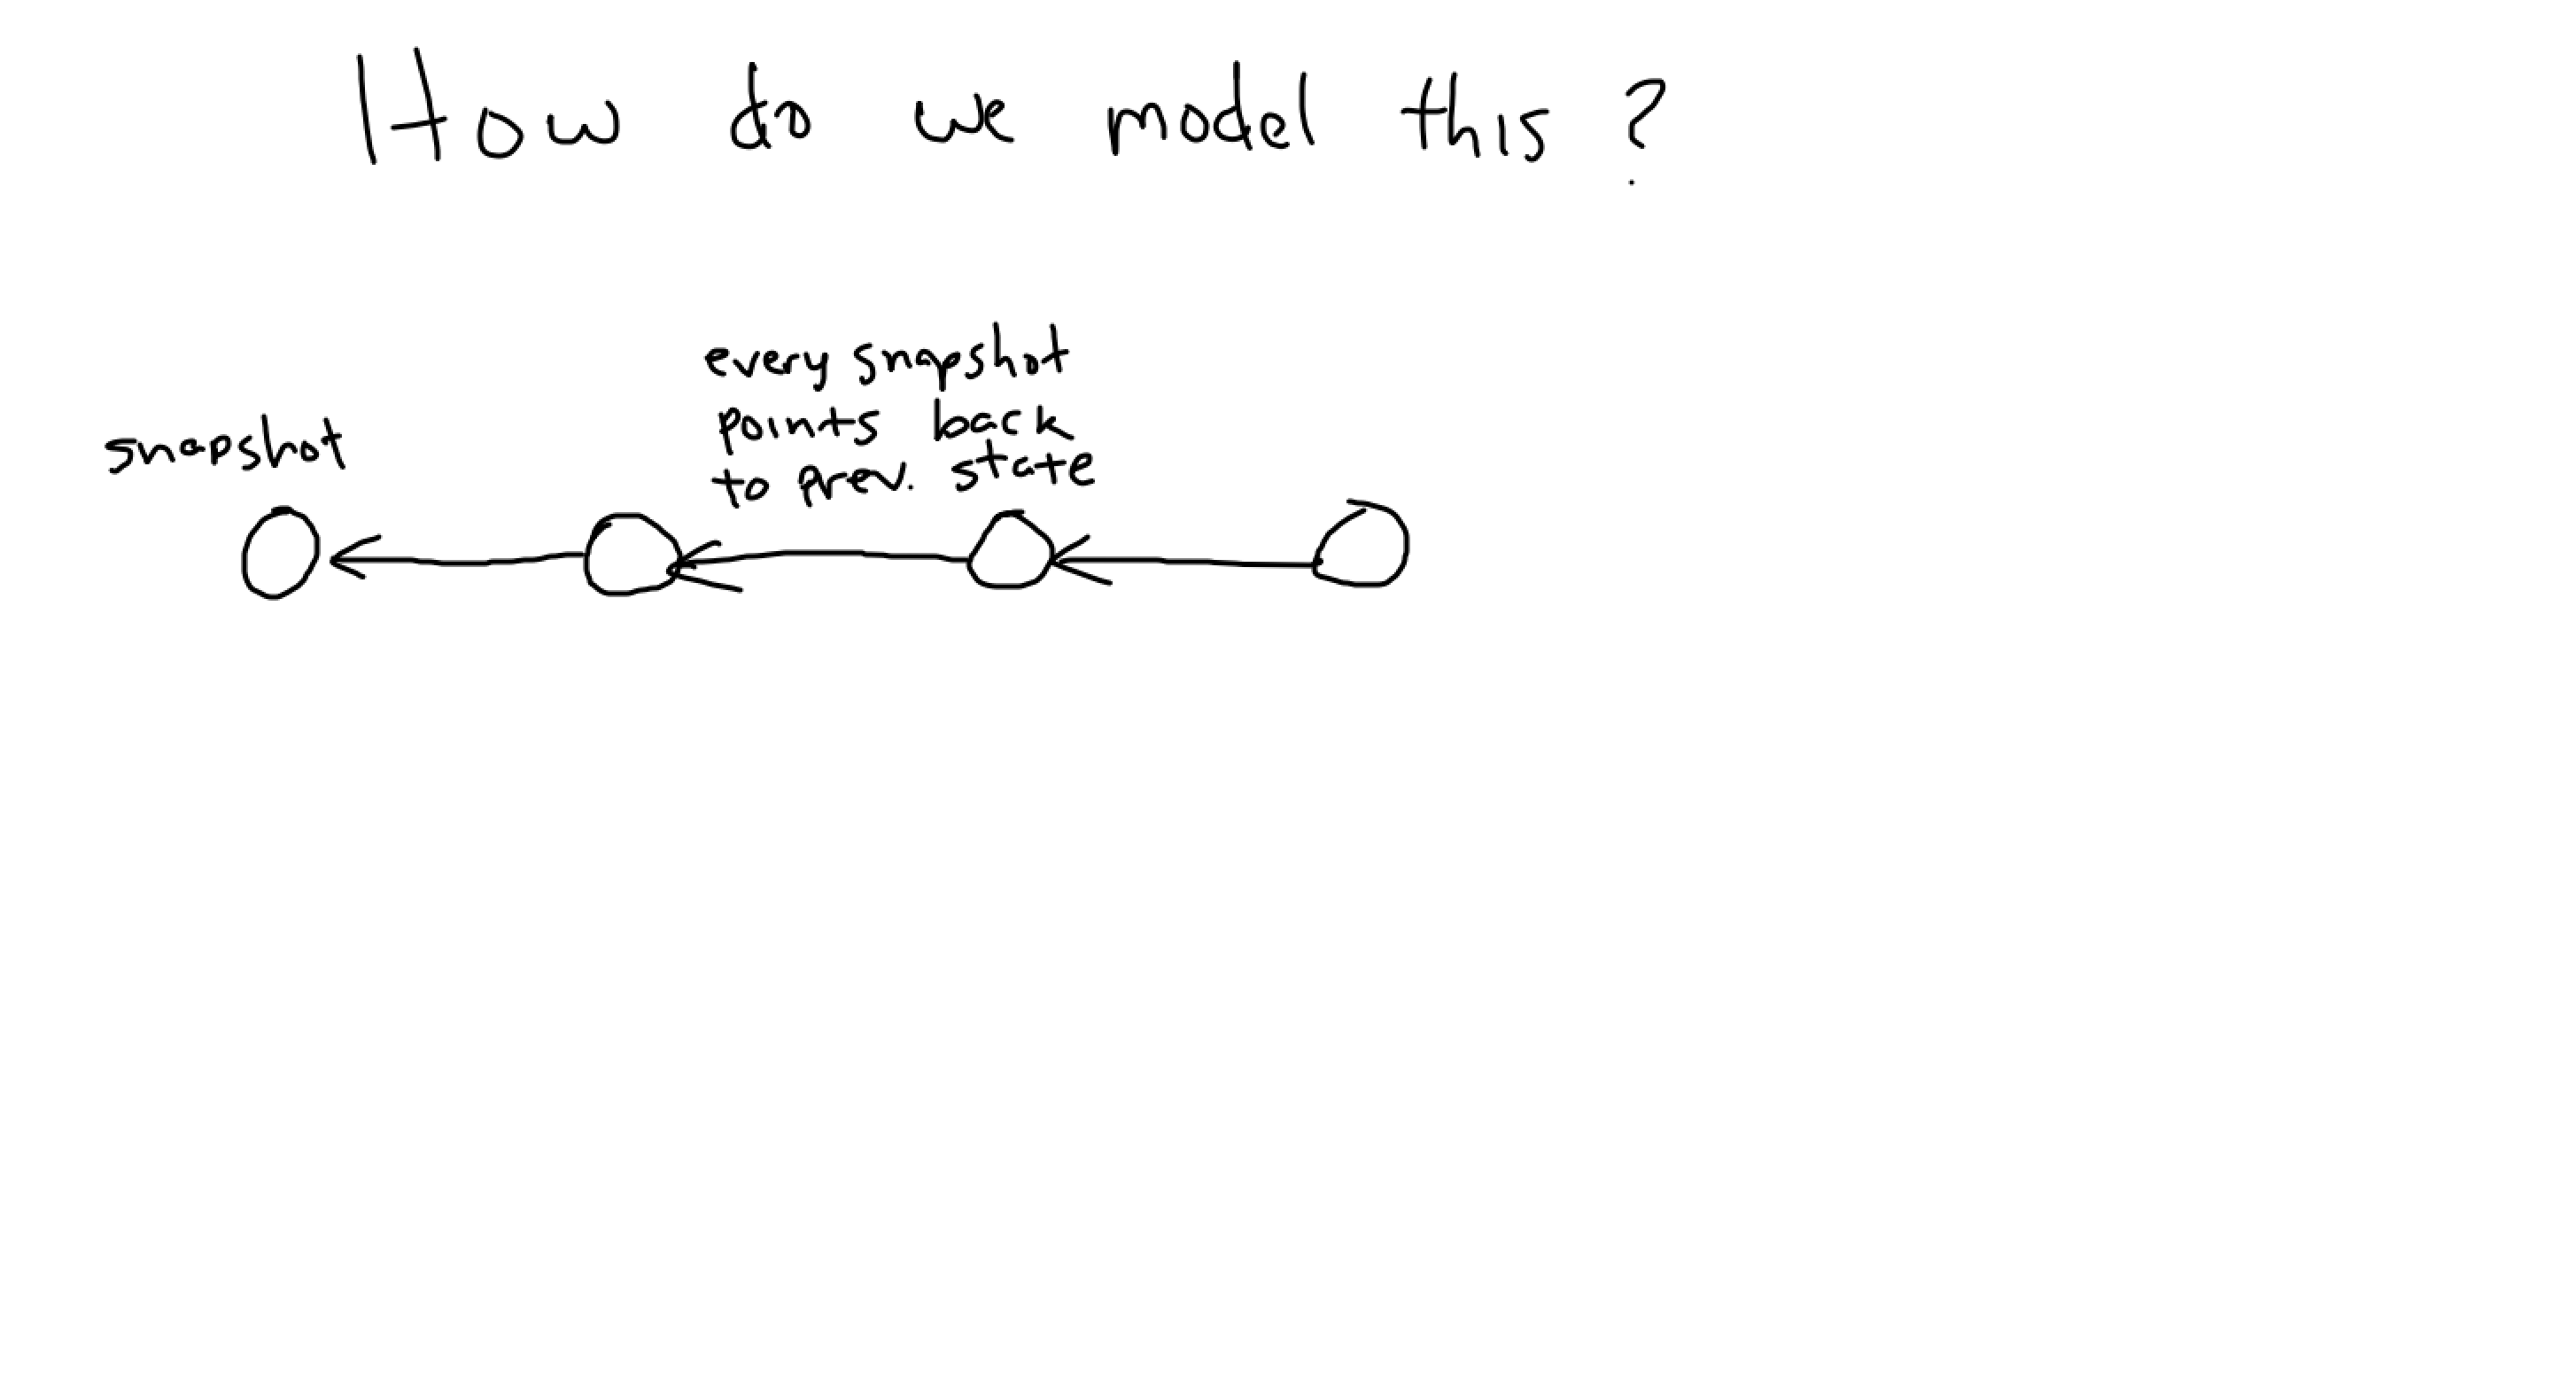
\includegraphics[scale=0.2]{git_model2a.png}
\end{figure}

\end{frame}


% --- Slide

\begin{frame}[fragile]
\frametitle{The Git Model}

\begin{figure}[htp]
 \centering
 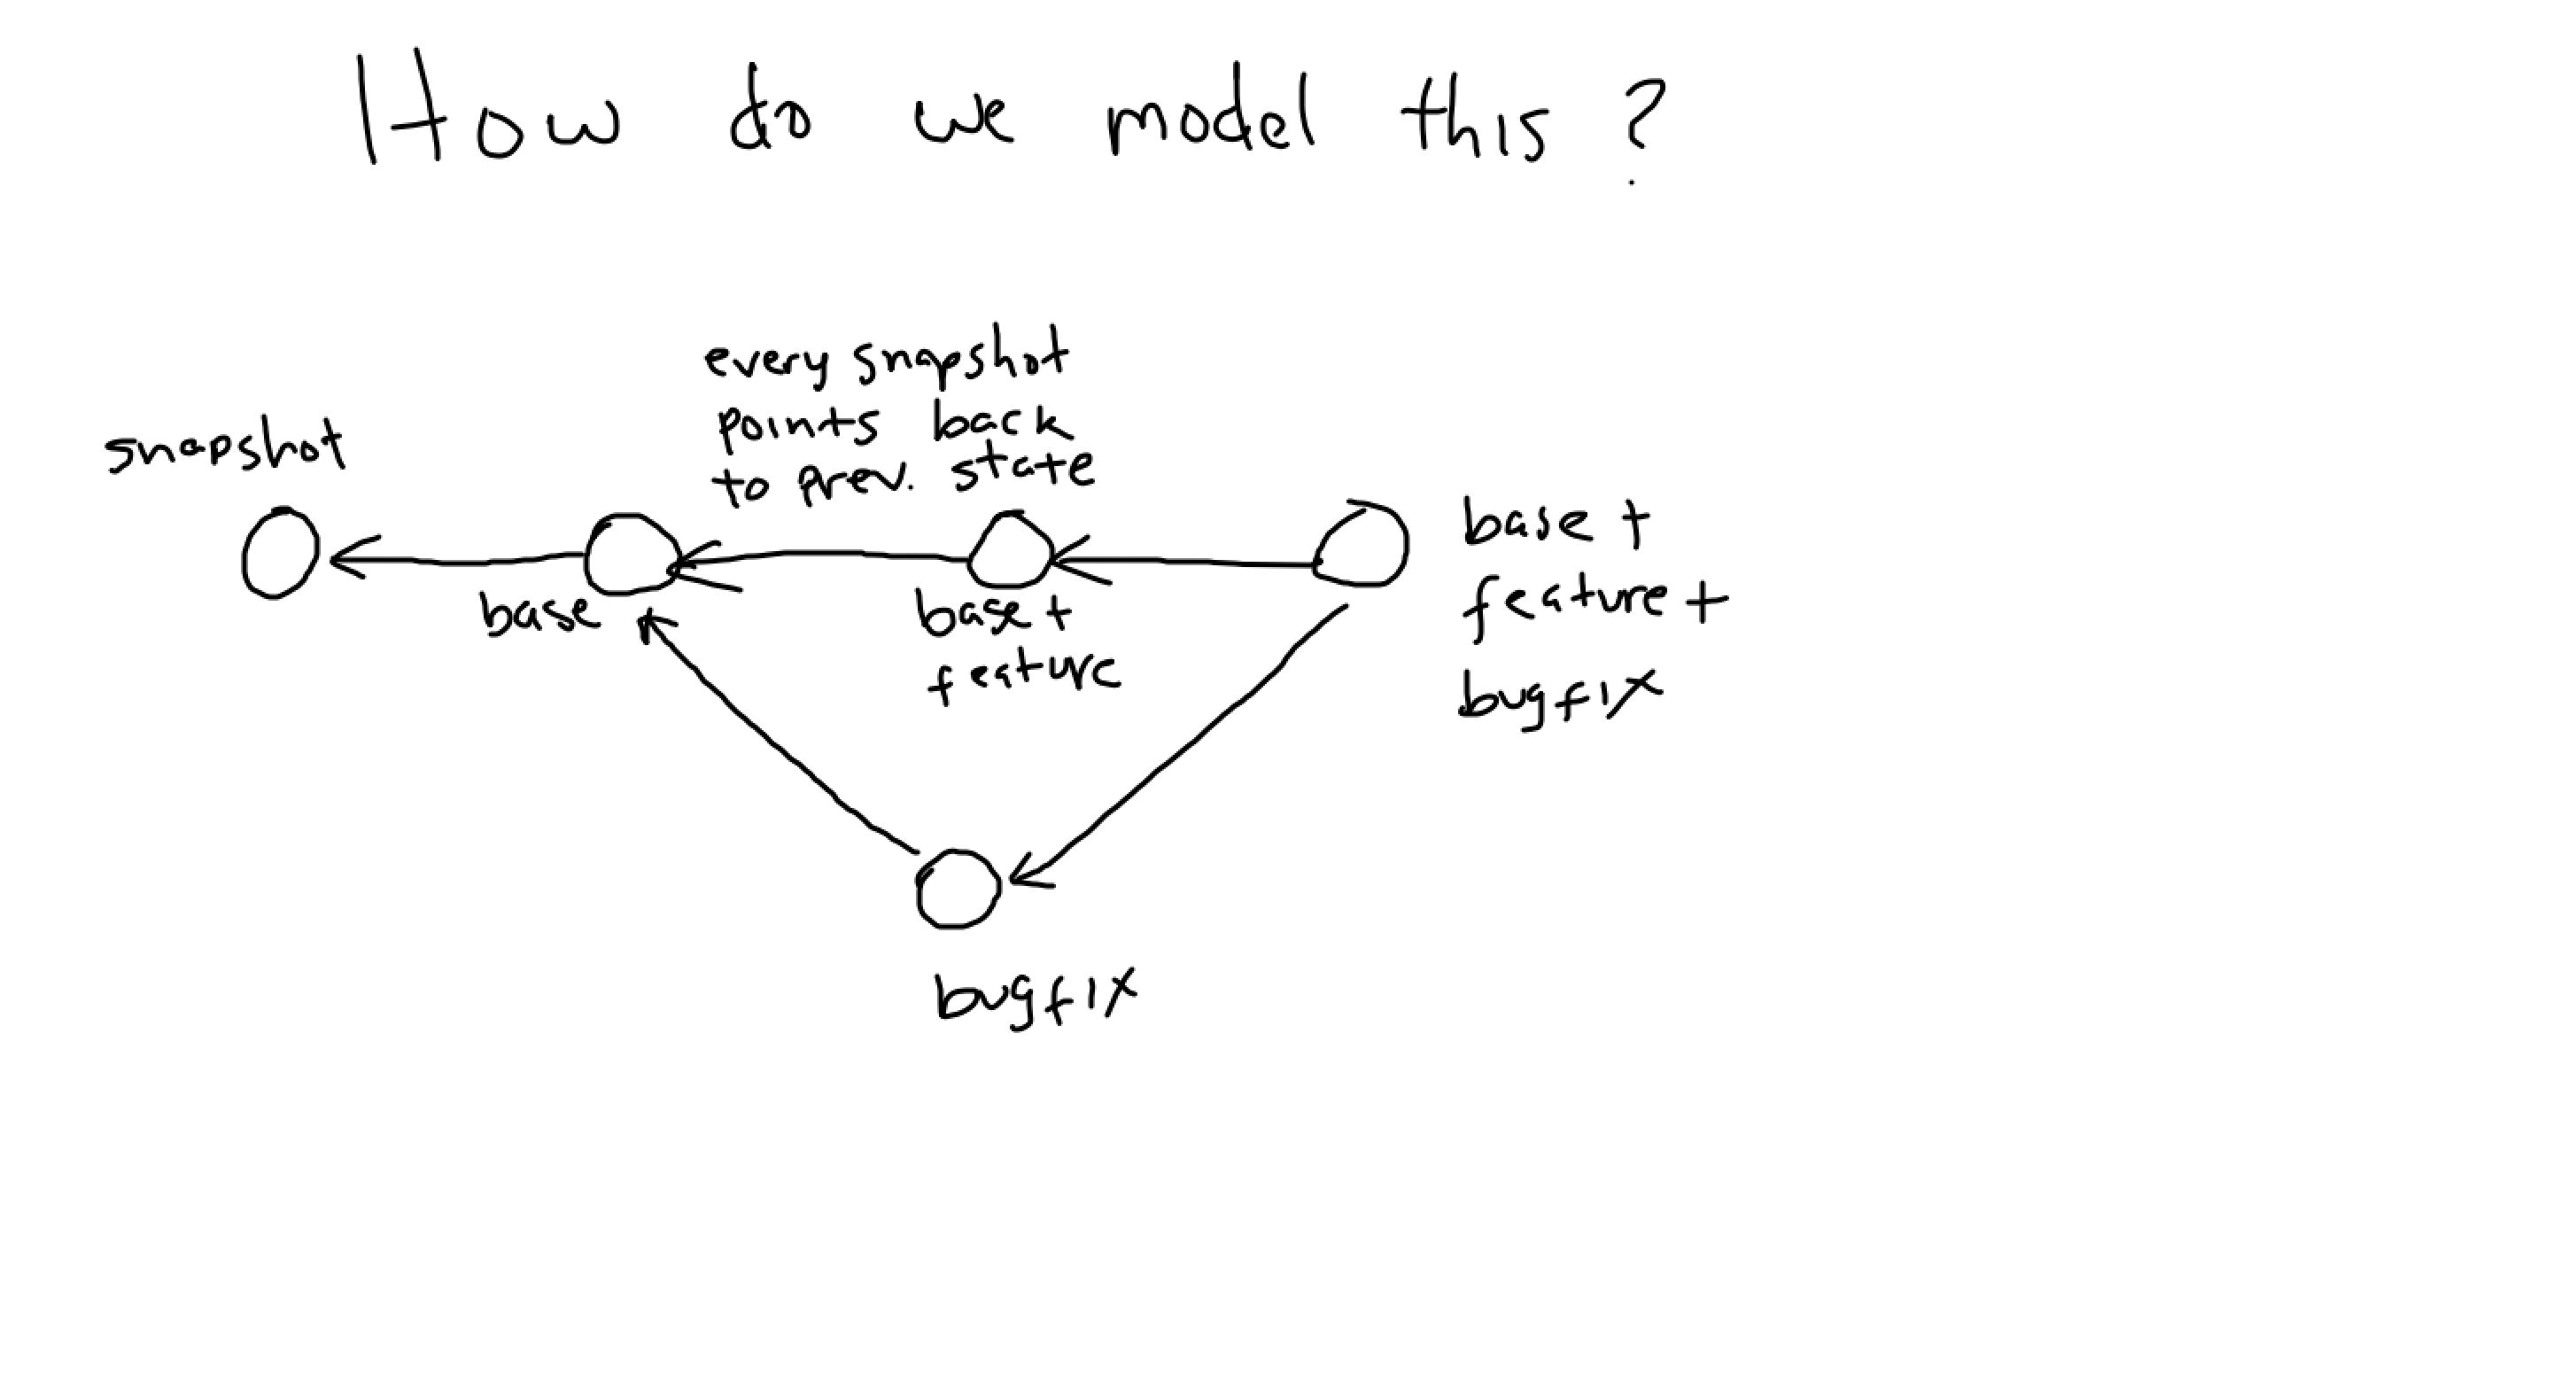
\includegraphics[scale=0.2]{git_model2b.png}
\end{figure}

\end{frame}


% --- Slide

\begin{frame}[fragile]
\frametitle{The Git Model}

\begin{figure}[htp]
 \centering
 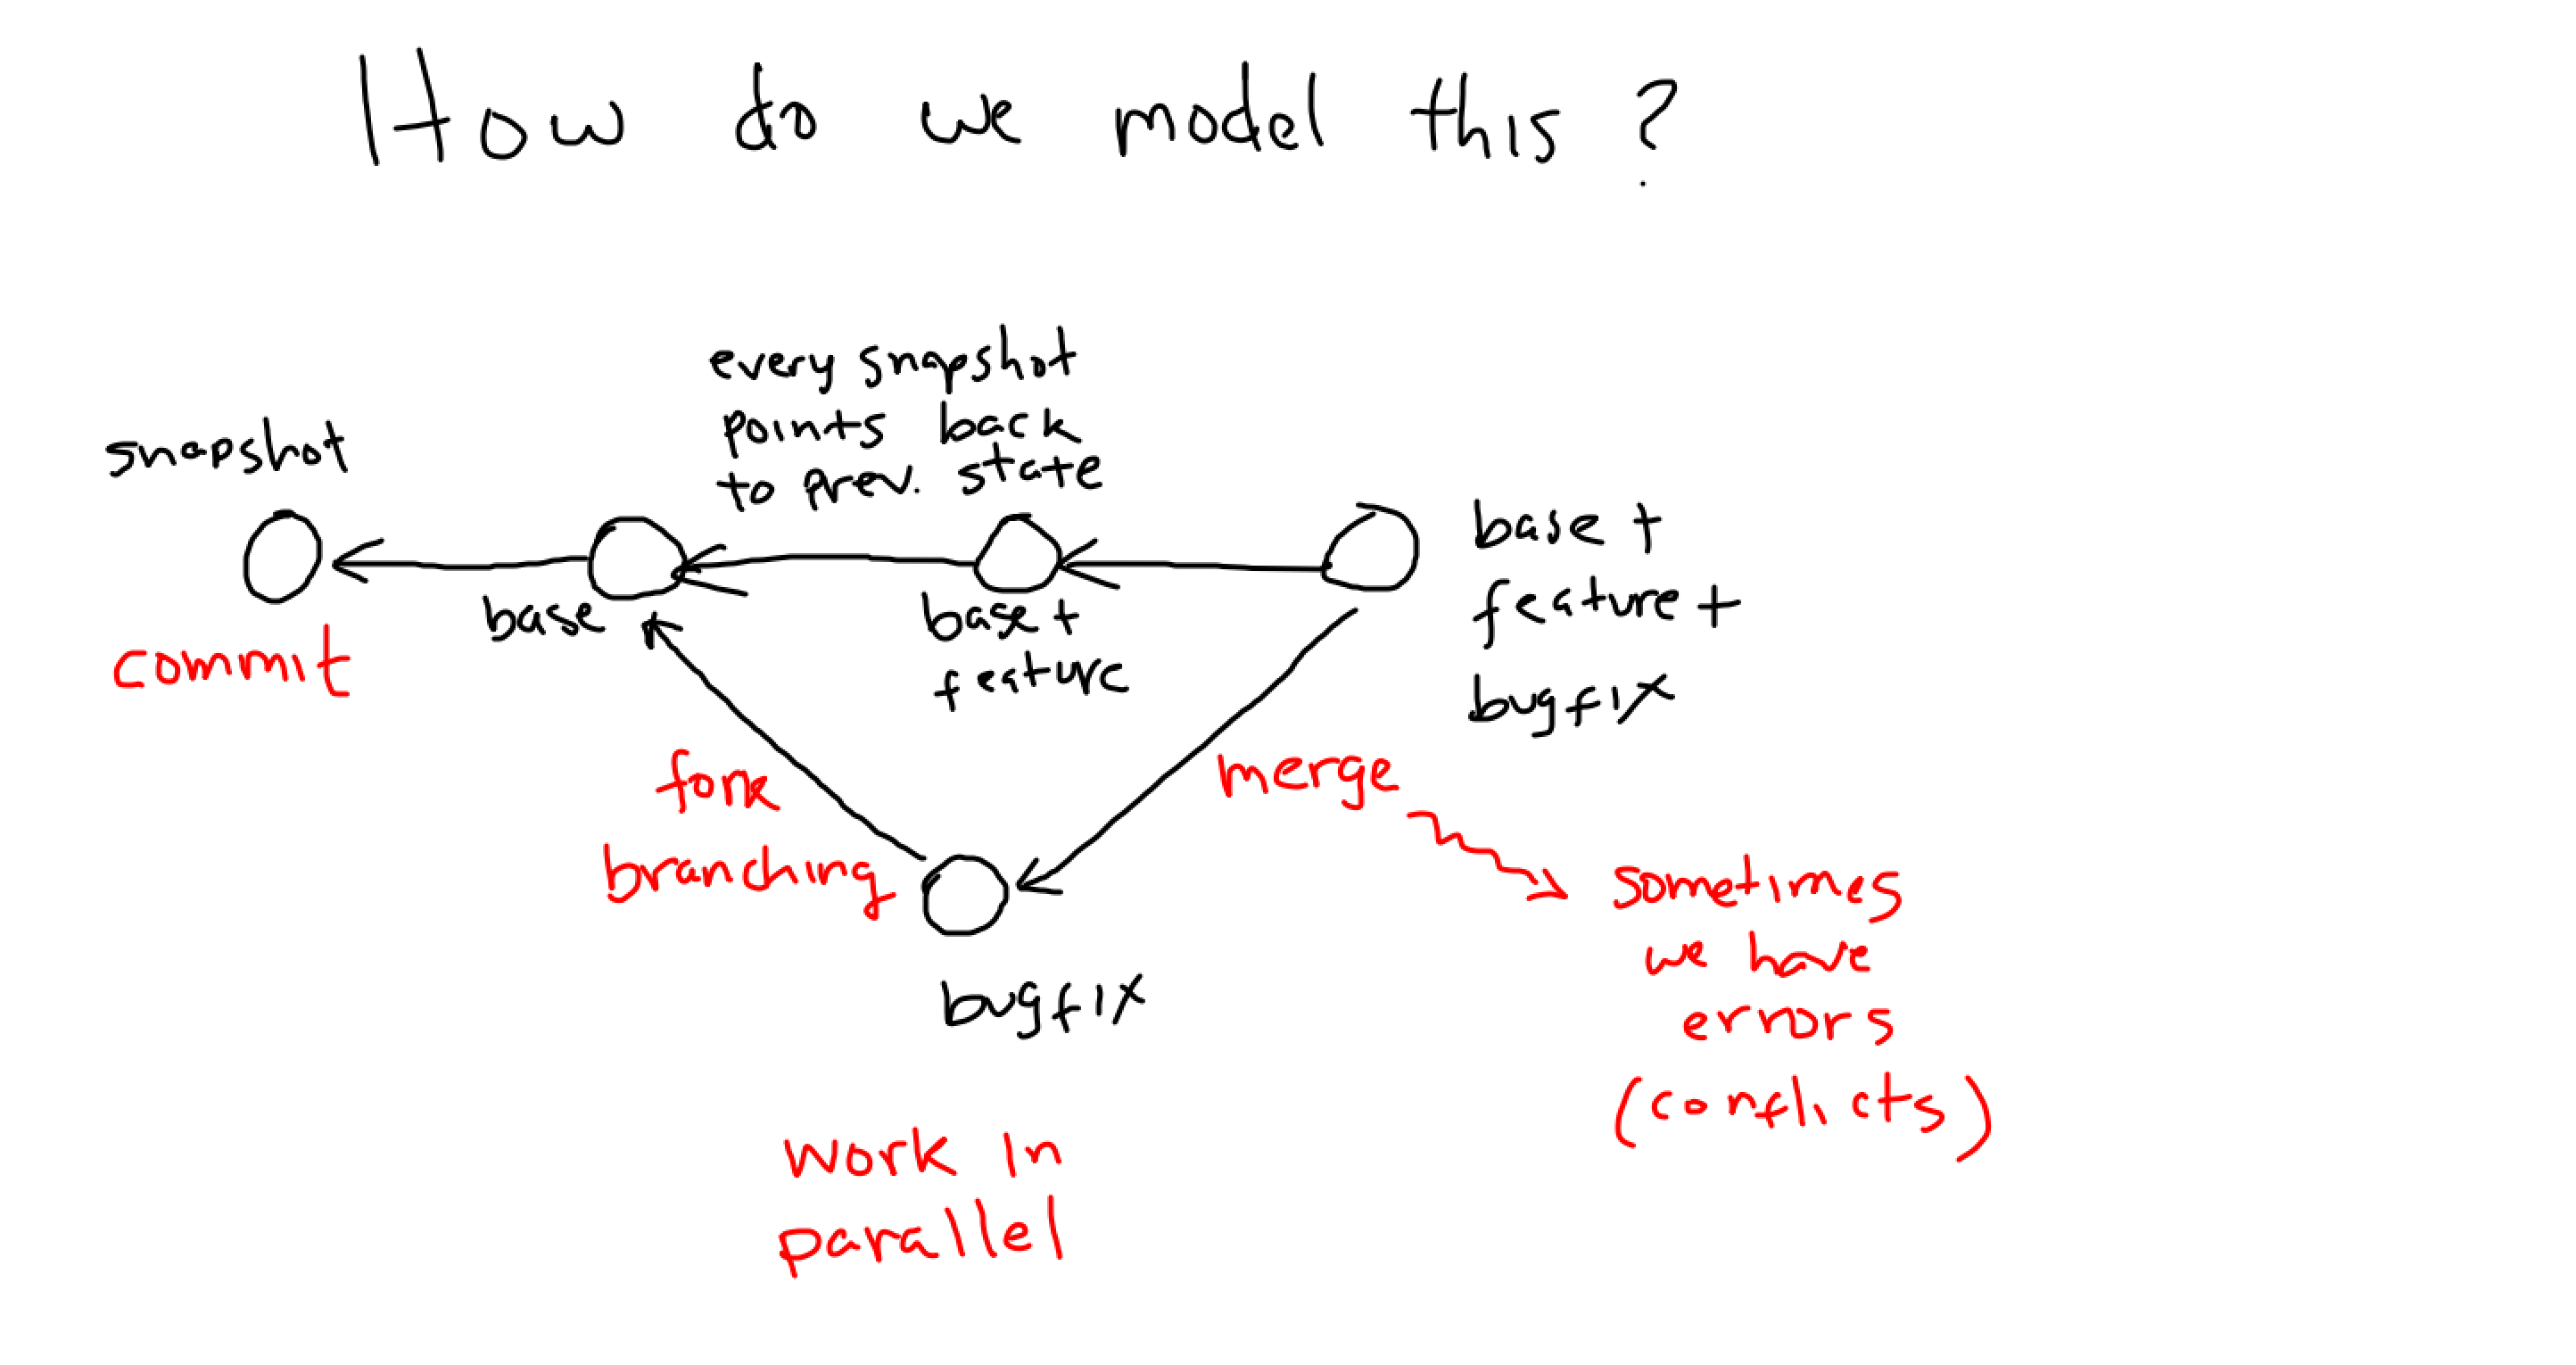
\includegraphics[scale=0.2]{git_model2.png}
\end{figure}

\end{frame}



% --- Slide

\begin{frame}[fragile]
\frametitle{The Git Model}

\begin{figure}[htp]
 \centering
 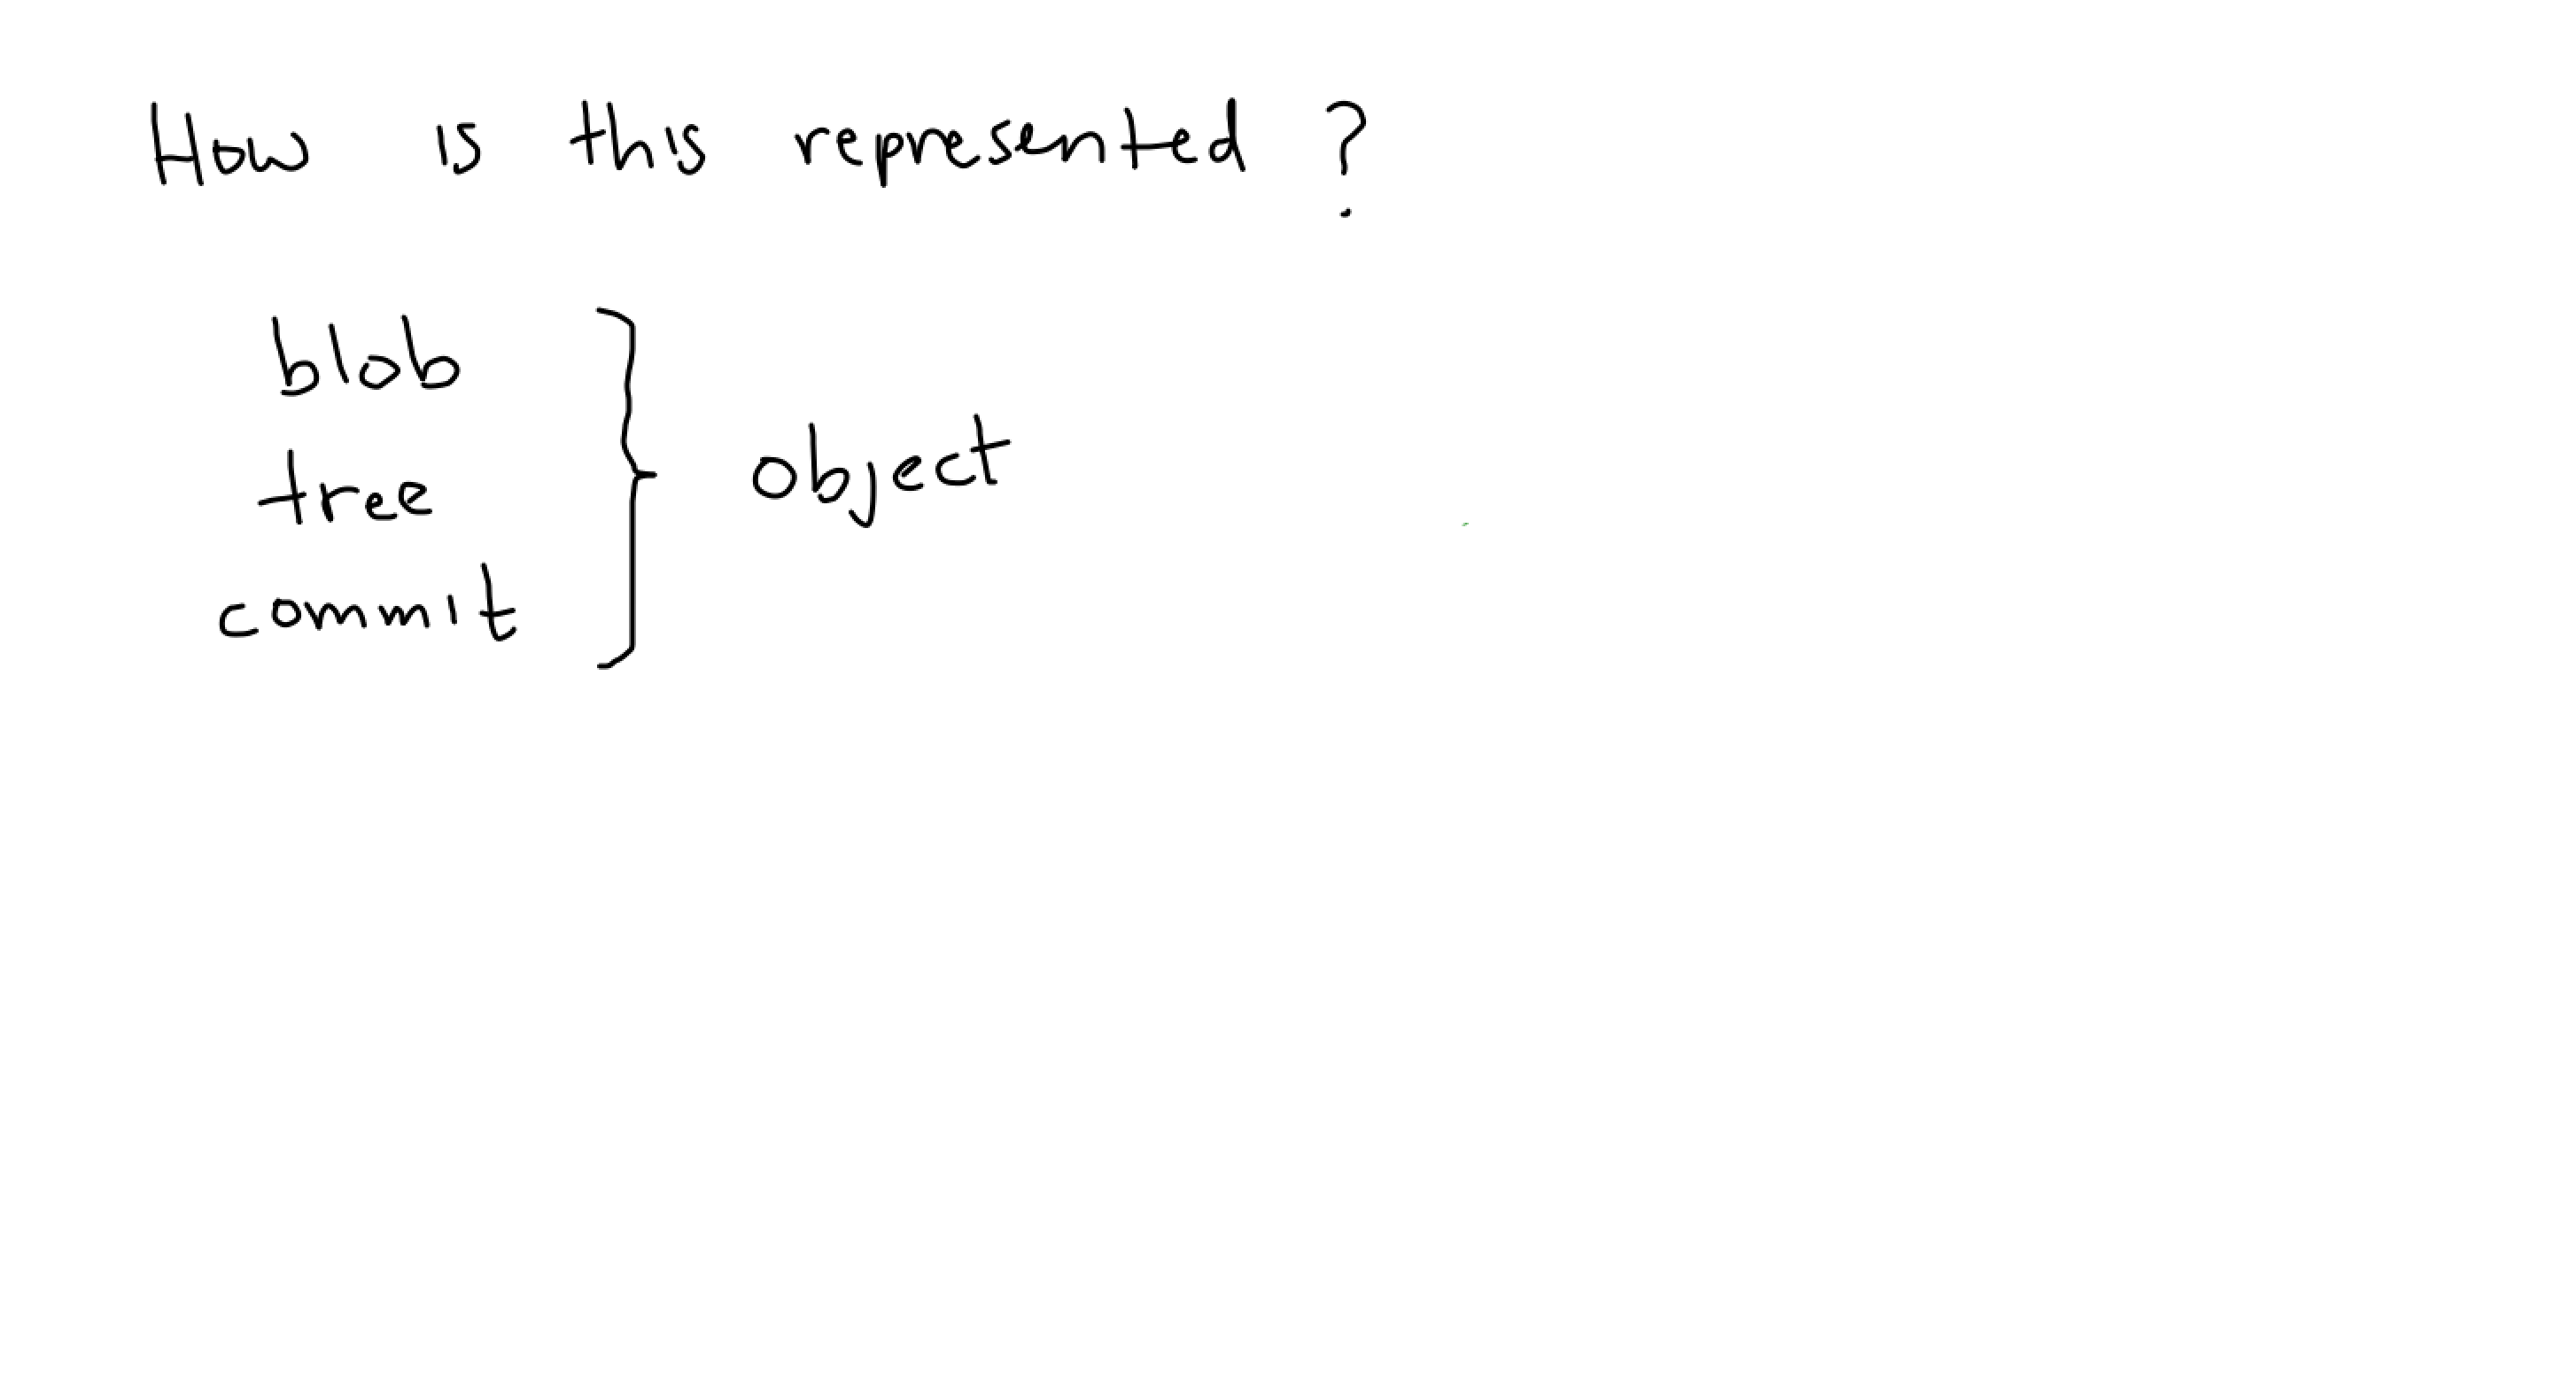
\includegraphics[scale=0.2]{git_model3a.png}
\end{figure}

\end{frame}



% --- Slide

\begin{frame}[fragile]
\frametitle{The Git Model}

\begin{figure}[htp]
 \centering
 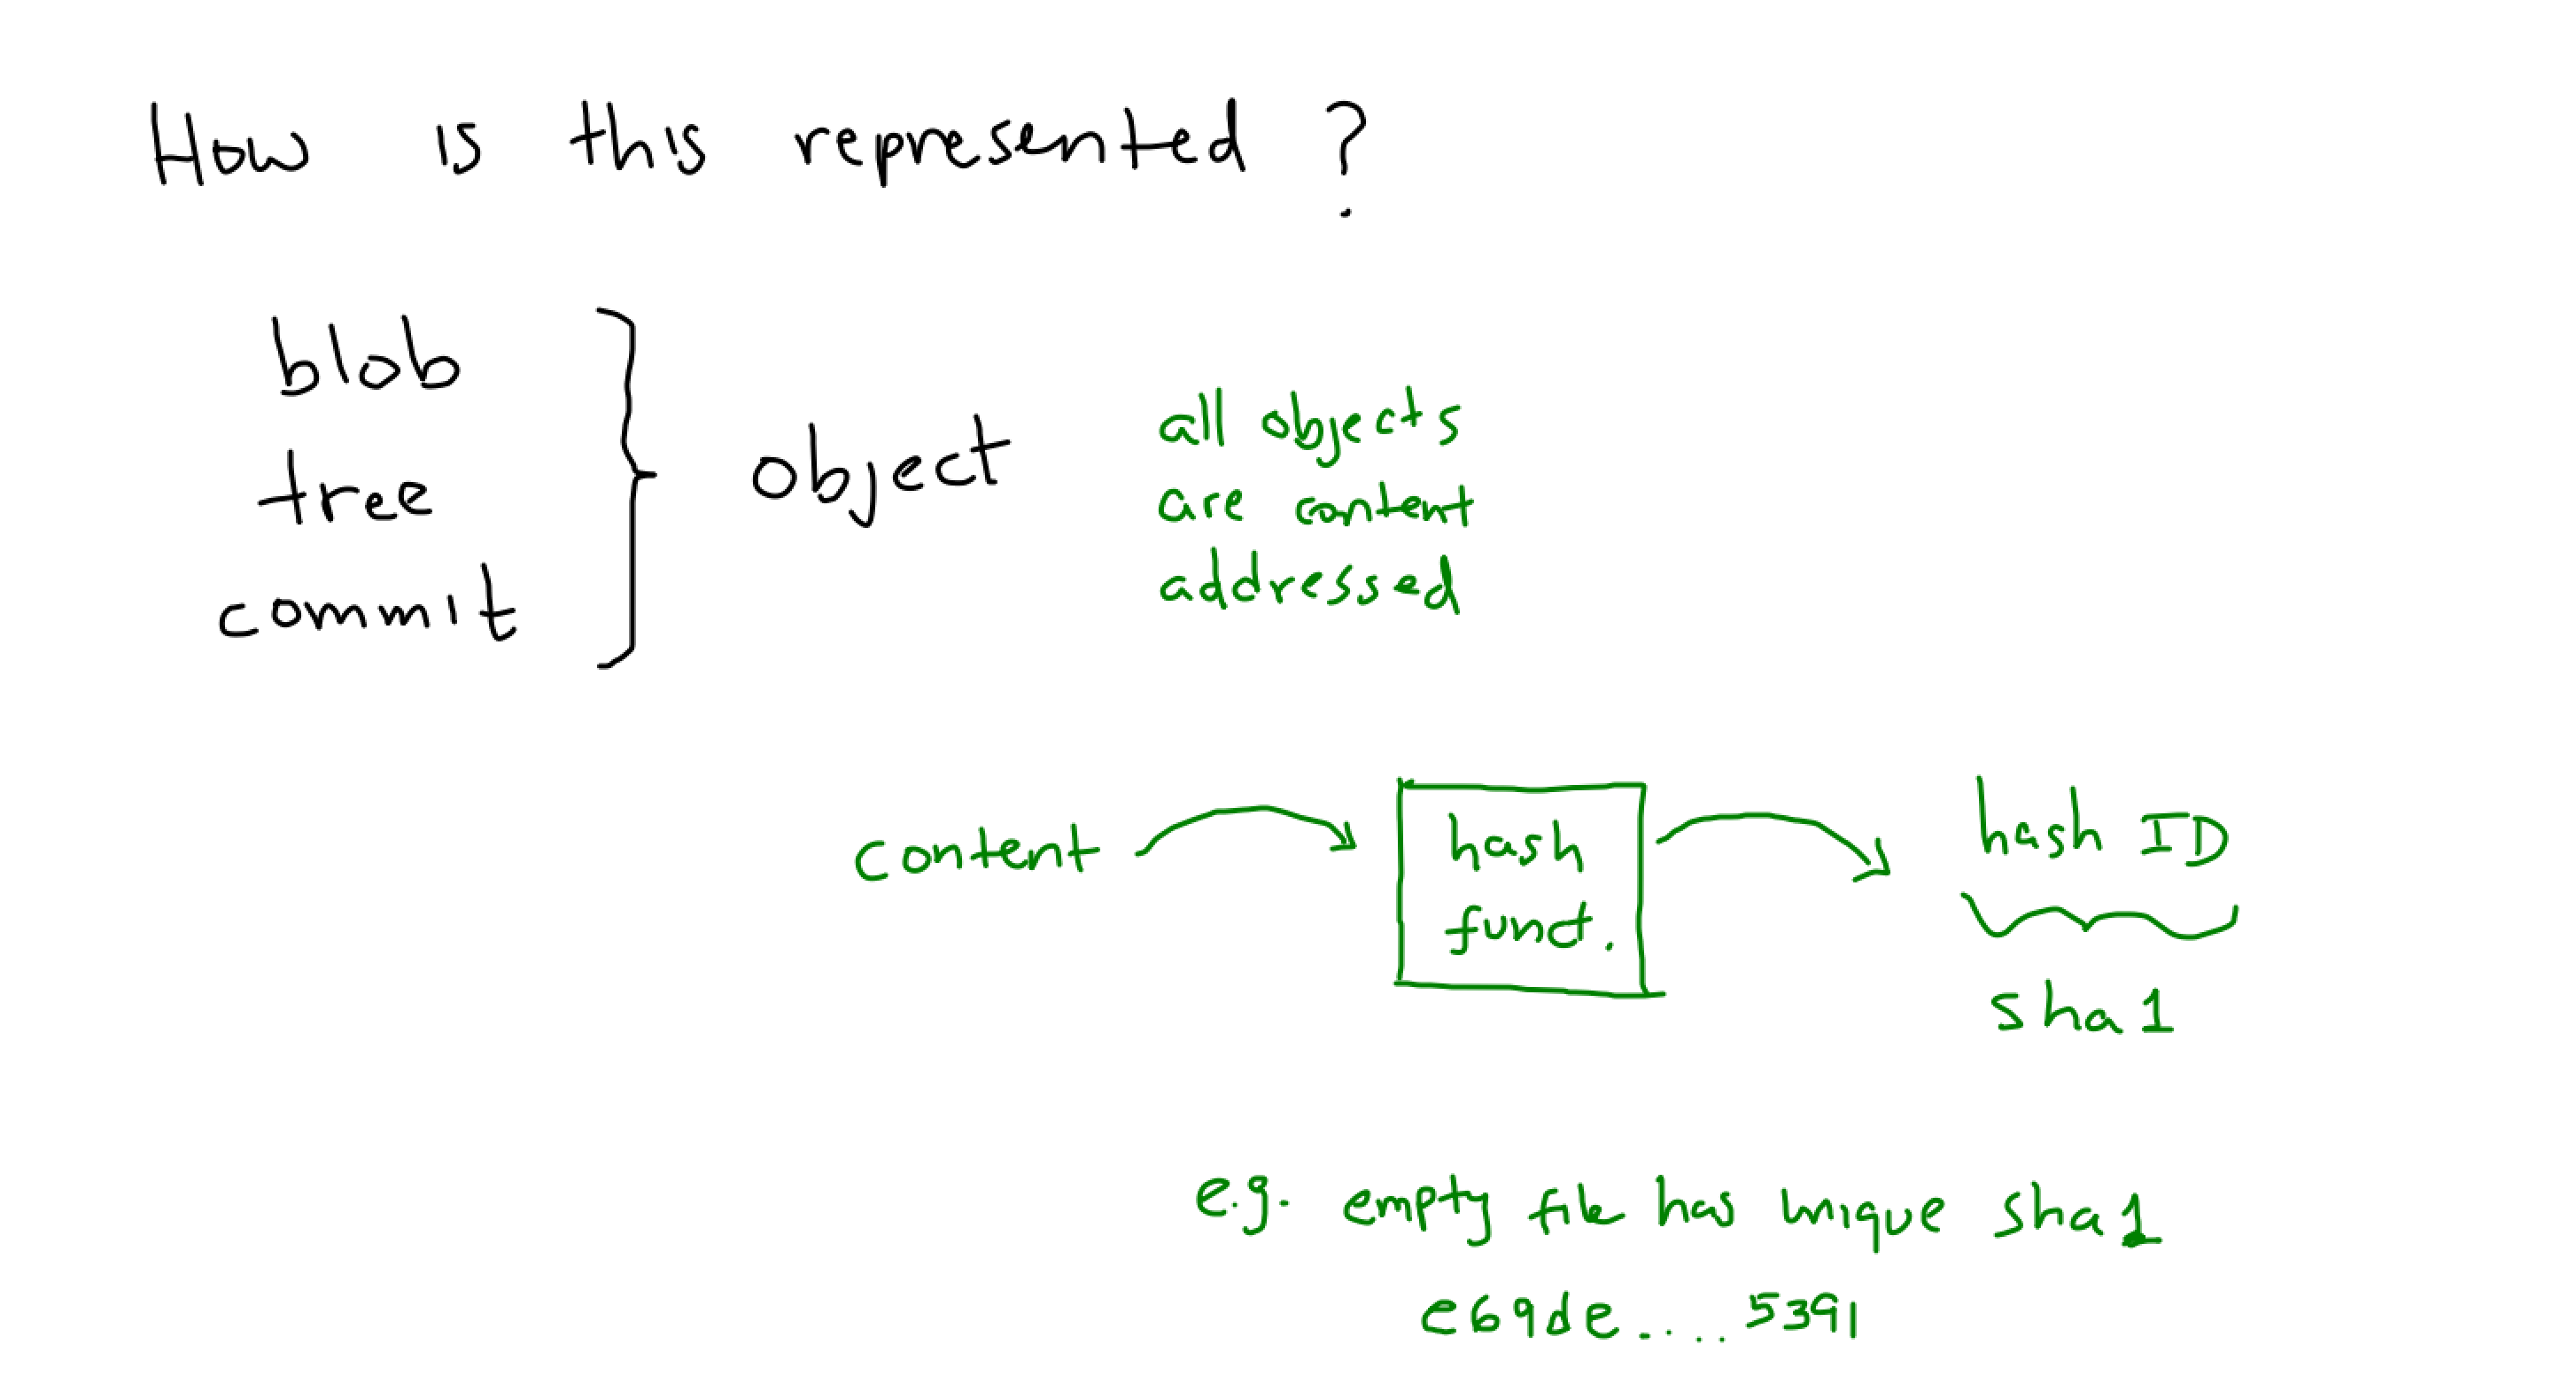
\includegraphics[scale=0.2]{git_model3b.png}
\end{figure}

\end{frame}



% --- Slide

\begin{frame}[fragile]
\frametitle{The Git Model}

\begin{figure}[htp]
 \centering
 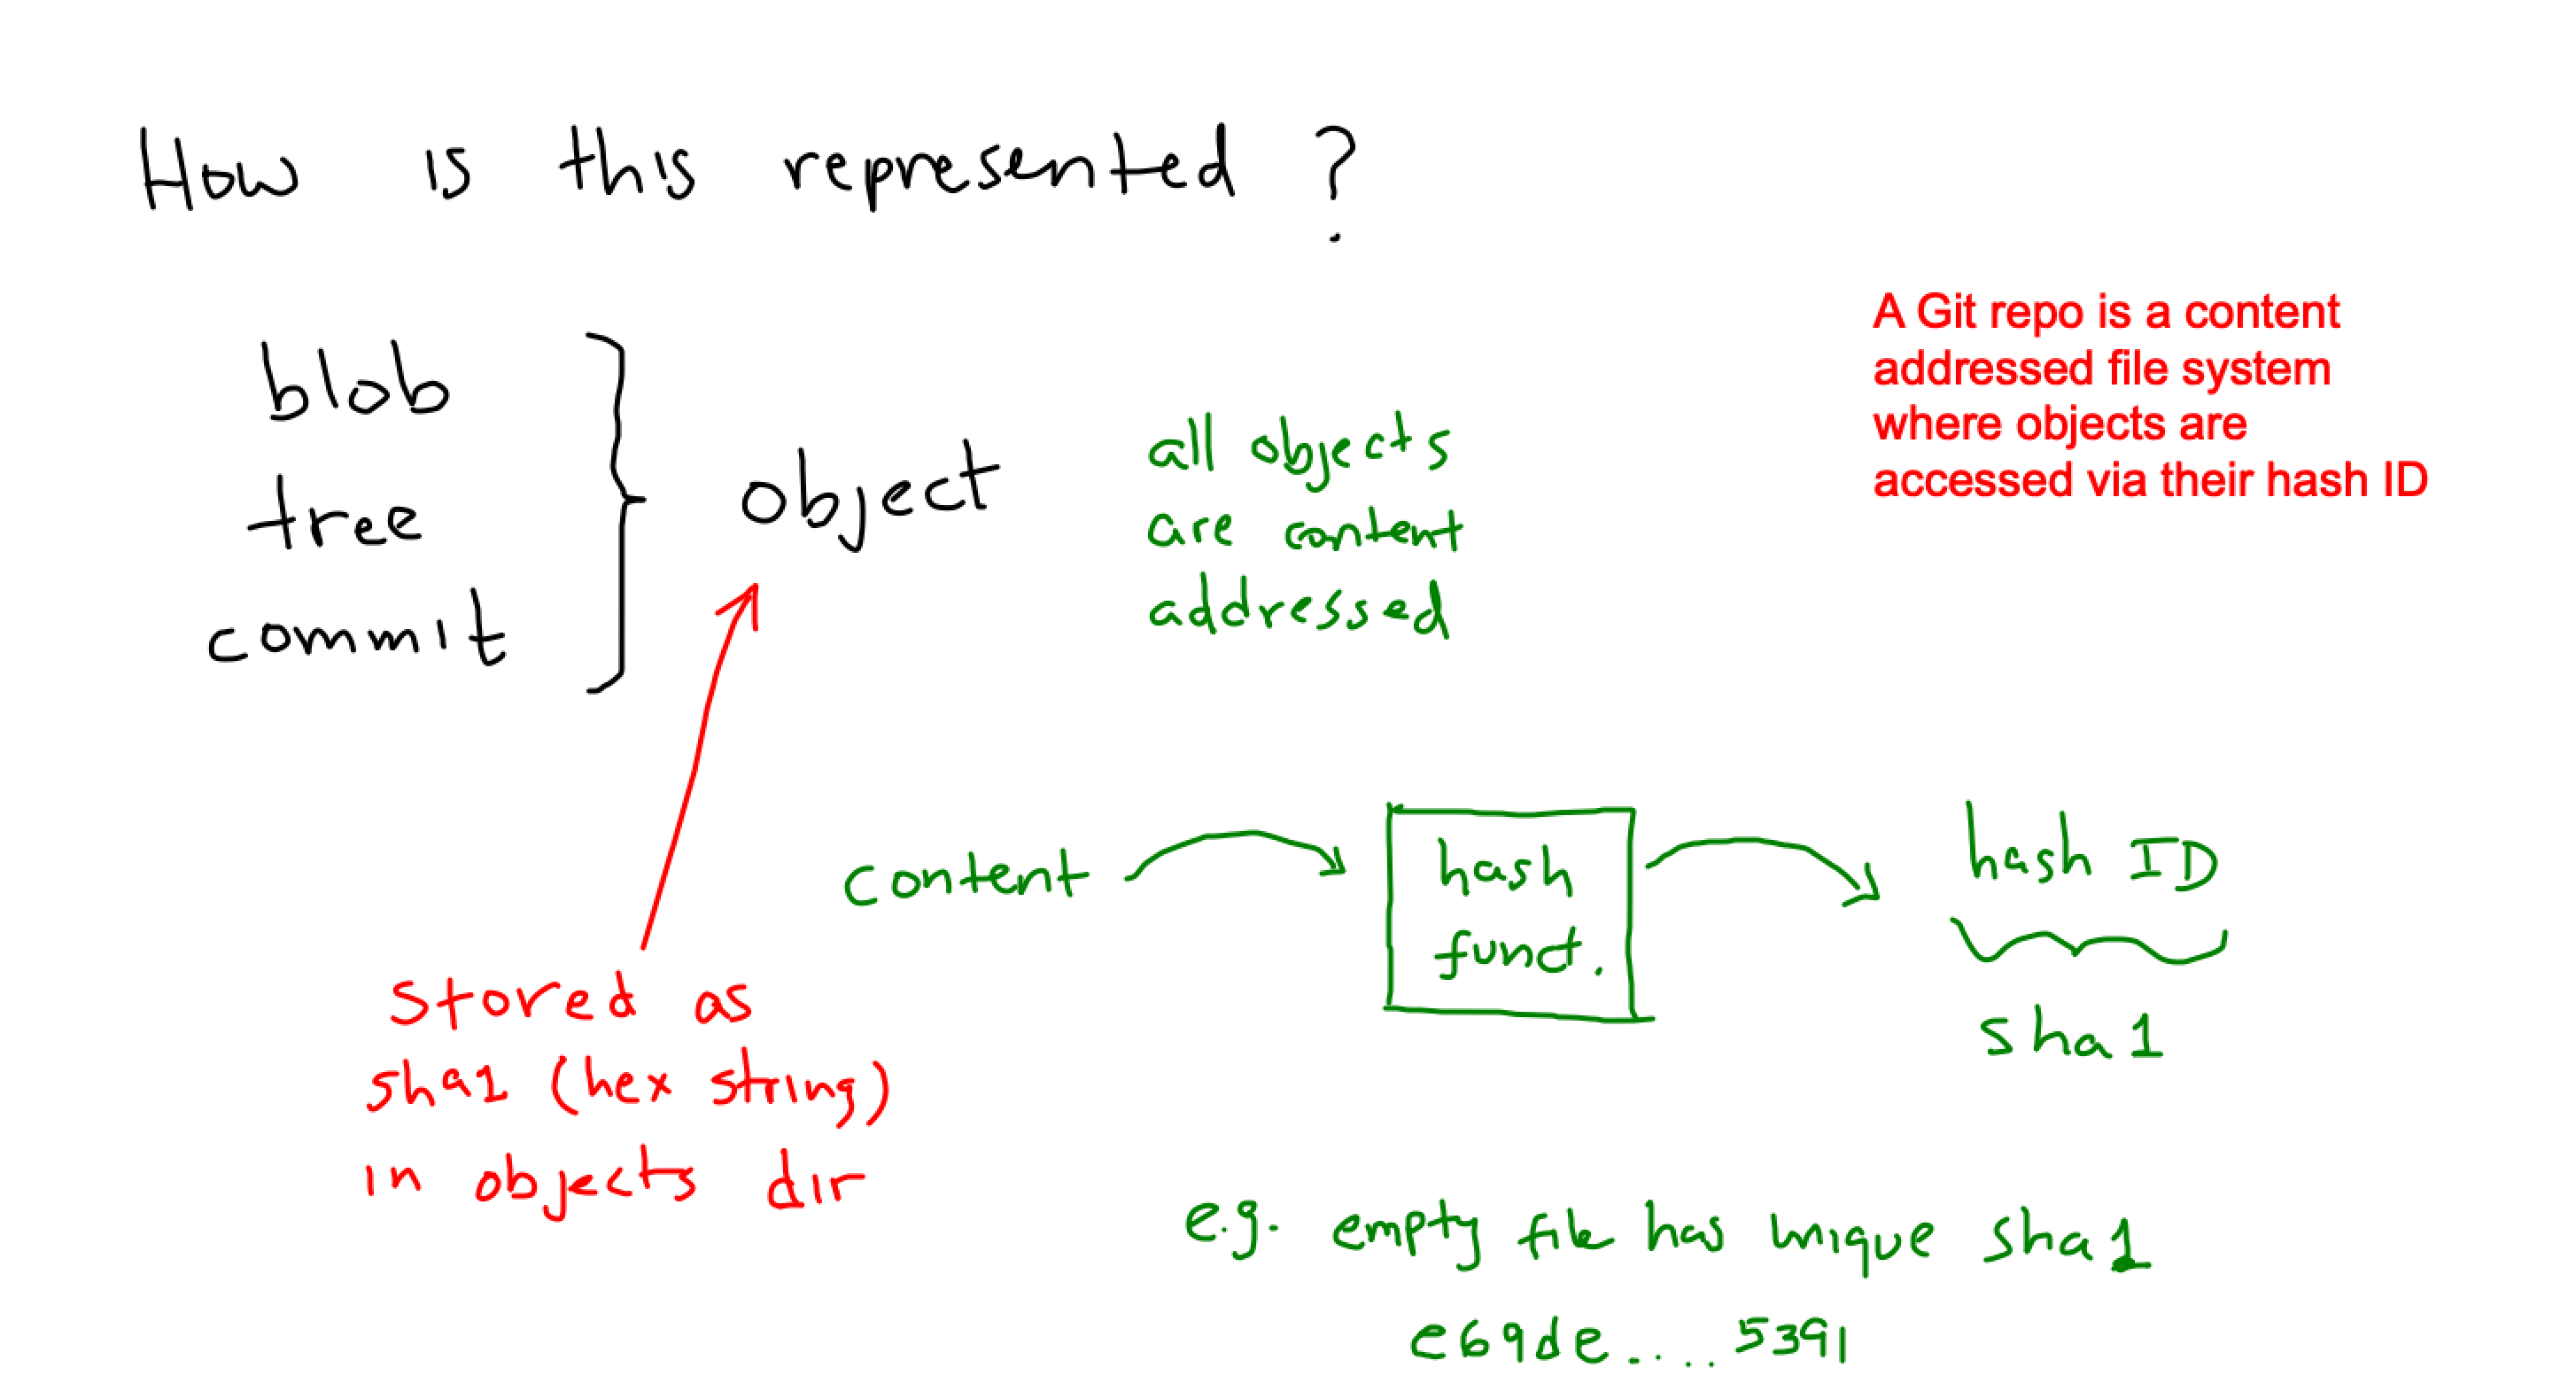
\includegraphics[scale=0.2]{git_model3.png}
\end{figure}

\end{frame}



% --- Slide

\begin{frame}[fragile]
\frametitle{The Git model}

\begin{figure}[htp]
 \centering
 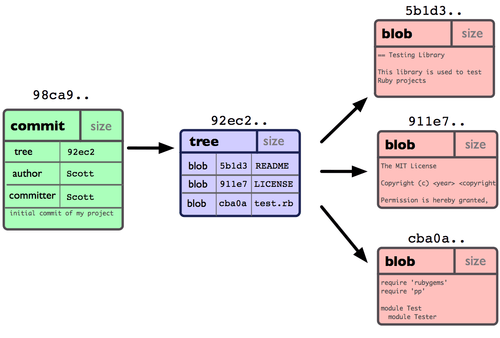
\includegraphics[scale=0.45]{gitInternals1.png}
\end{figure}

%Object types:
%commit: author, message, pointer to a tree of changes
%tree: pointer to file names, content, other trees
%blob: data


%First commit ? no parent

% what Git does when you run the git add and git commit commands ? it stores blobs for the files that have changed, updates the index, writes out trees, and writes commit objects that reference the top-level trees and the commits that came immediately before them. 

%These three main Git objects ? the blob, the tree, and the commit ? are initially stored as separate files in your .git/objects directory.

\end{frame}



% --- Slide

\begin{frame}[fragile]
\frametitle{The Git Setup}

\begin{figure}[htp]
 \centering
 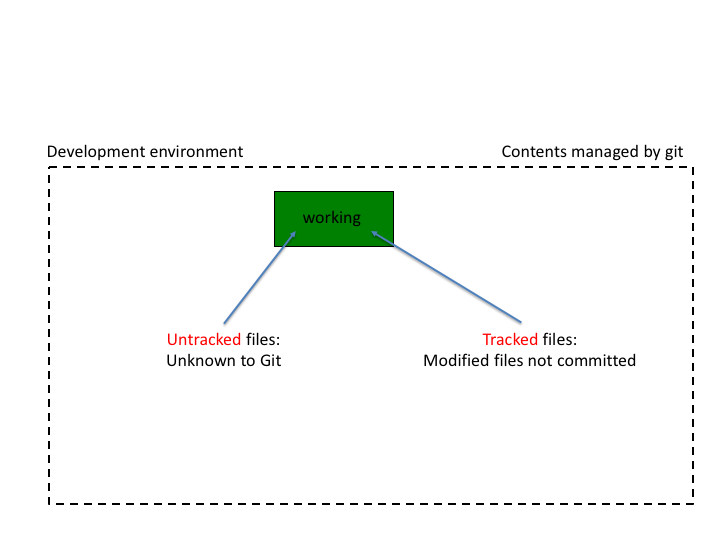
\includegraphics[scale=0.35]{gitB.png}
\end{figure}

%The general drawing contains 4 areas distributed as follows:

%The development environment with:
%Working directory
%Staging area or index
%Local repository
%A server with:
%Remote repository


\end{frame}


% --- Slide

\begin{frame}[fragile]
\frametitle{Branching}
Commits are repository snapshots
\begin{figure}[htp]
 \centering
 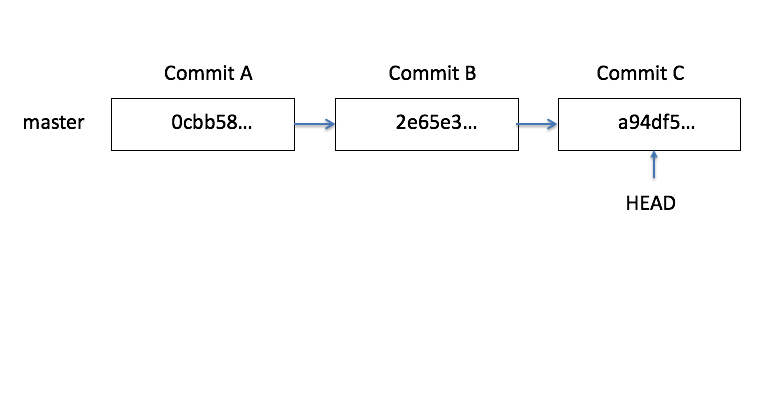
\includegraphics[scale=0.35]{branch1.png}
\end{figure}

% Git is a database of references
%% commits all reference their parent

% Hex code of B (child of A) uses as a basis hex code of parent A => last commit has hex code that identifies entire history of repository


\end{frame}

% --- Slide

\begin{frame}[fragile]
\frametitle{Branching}
A branch is a pointer to  commit - not a full copy.
\begin{figure}[htp]
 \centering
 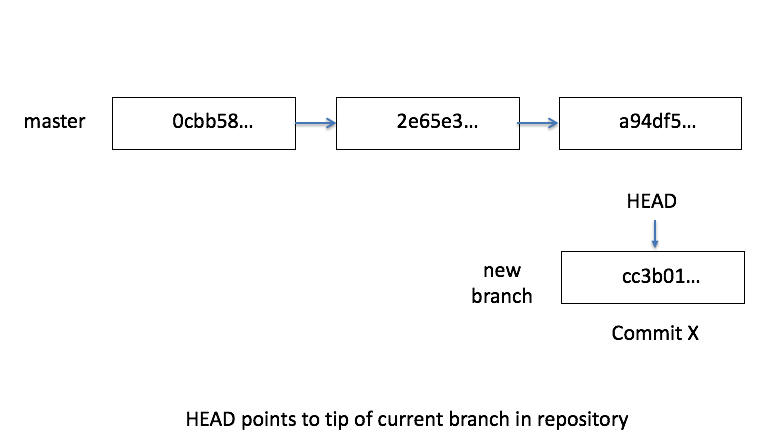
\includegraphics[scale=0.35]{branch2.png}
\end{figure}

% Git is a database of references
%% branches are named pointers to a commit
%% 'master' is the canonical mainline branch
%% HEAD is a special pointer to the latest commit
%%% moves automatically
% performing a clone/checkout starts at the current commit



\end{frame}

% --- Slide

\begin{frame}[fragile]
\frametitle{Branching}
Can have many branches
\begin{figure}[htp]
 \centering
 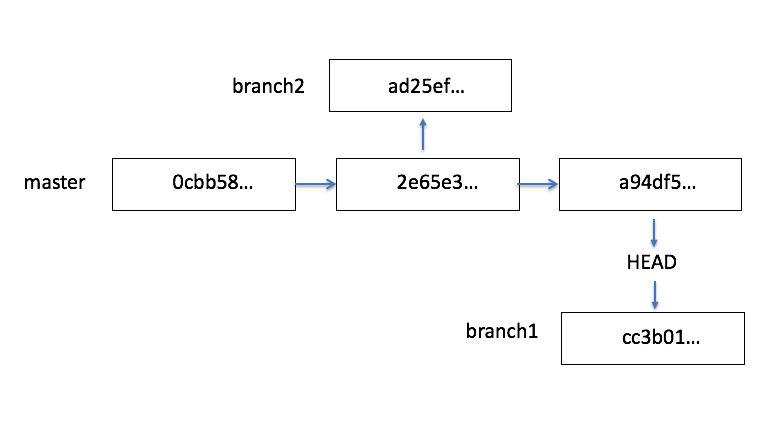
\includegraphics[scale=0.35]{branch3.png}
\end{figure}


\end{frame}

% --- Slide

\begin{frame}[fragile]
\frametitle{Merging}
We have two branches
\begin{figure}[htp]
 \centering
 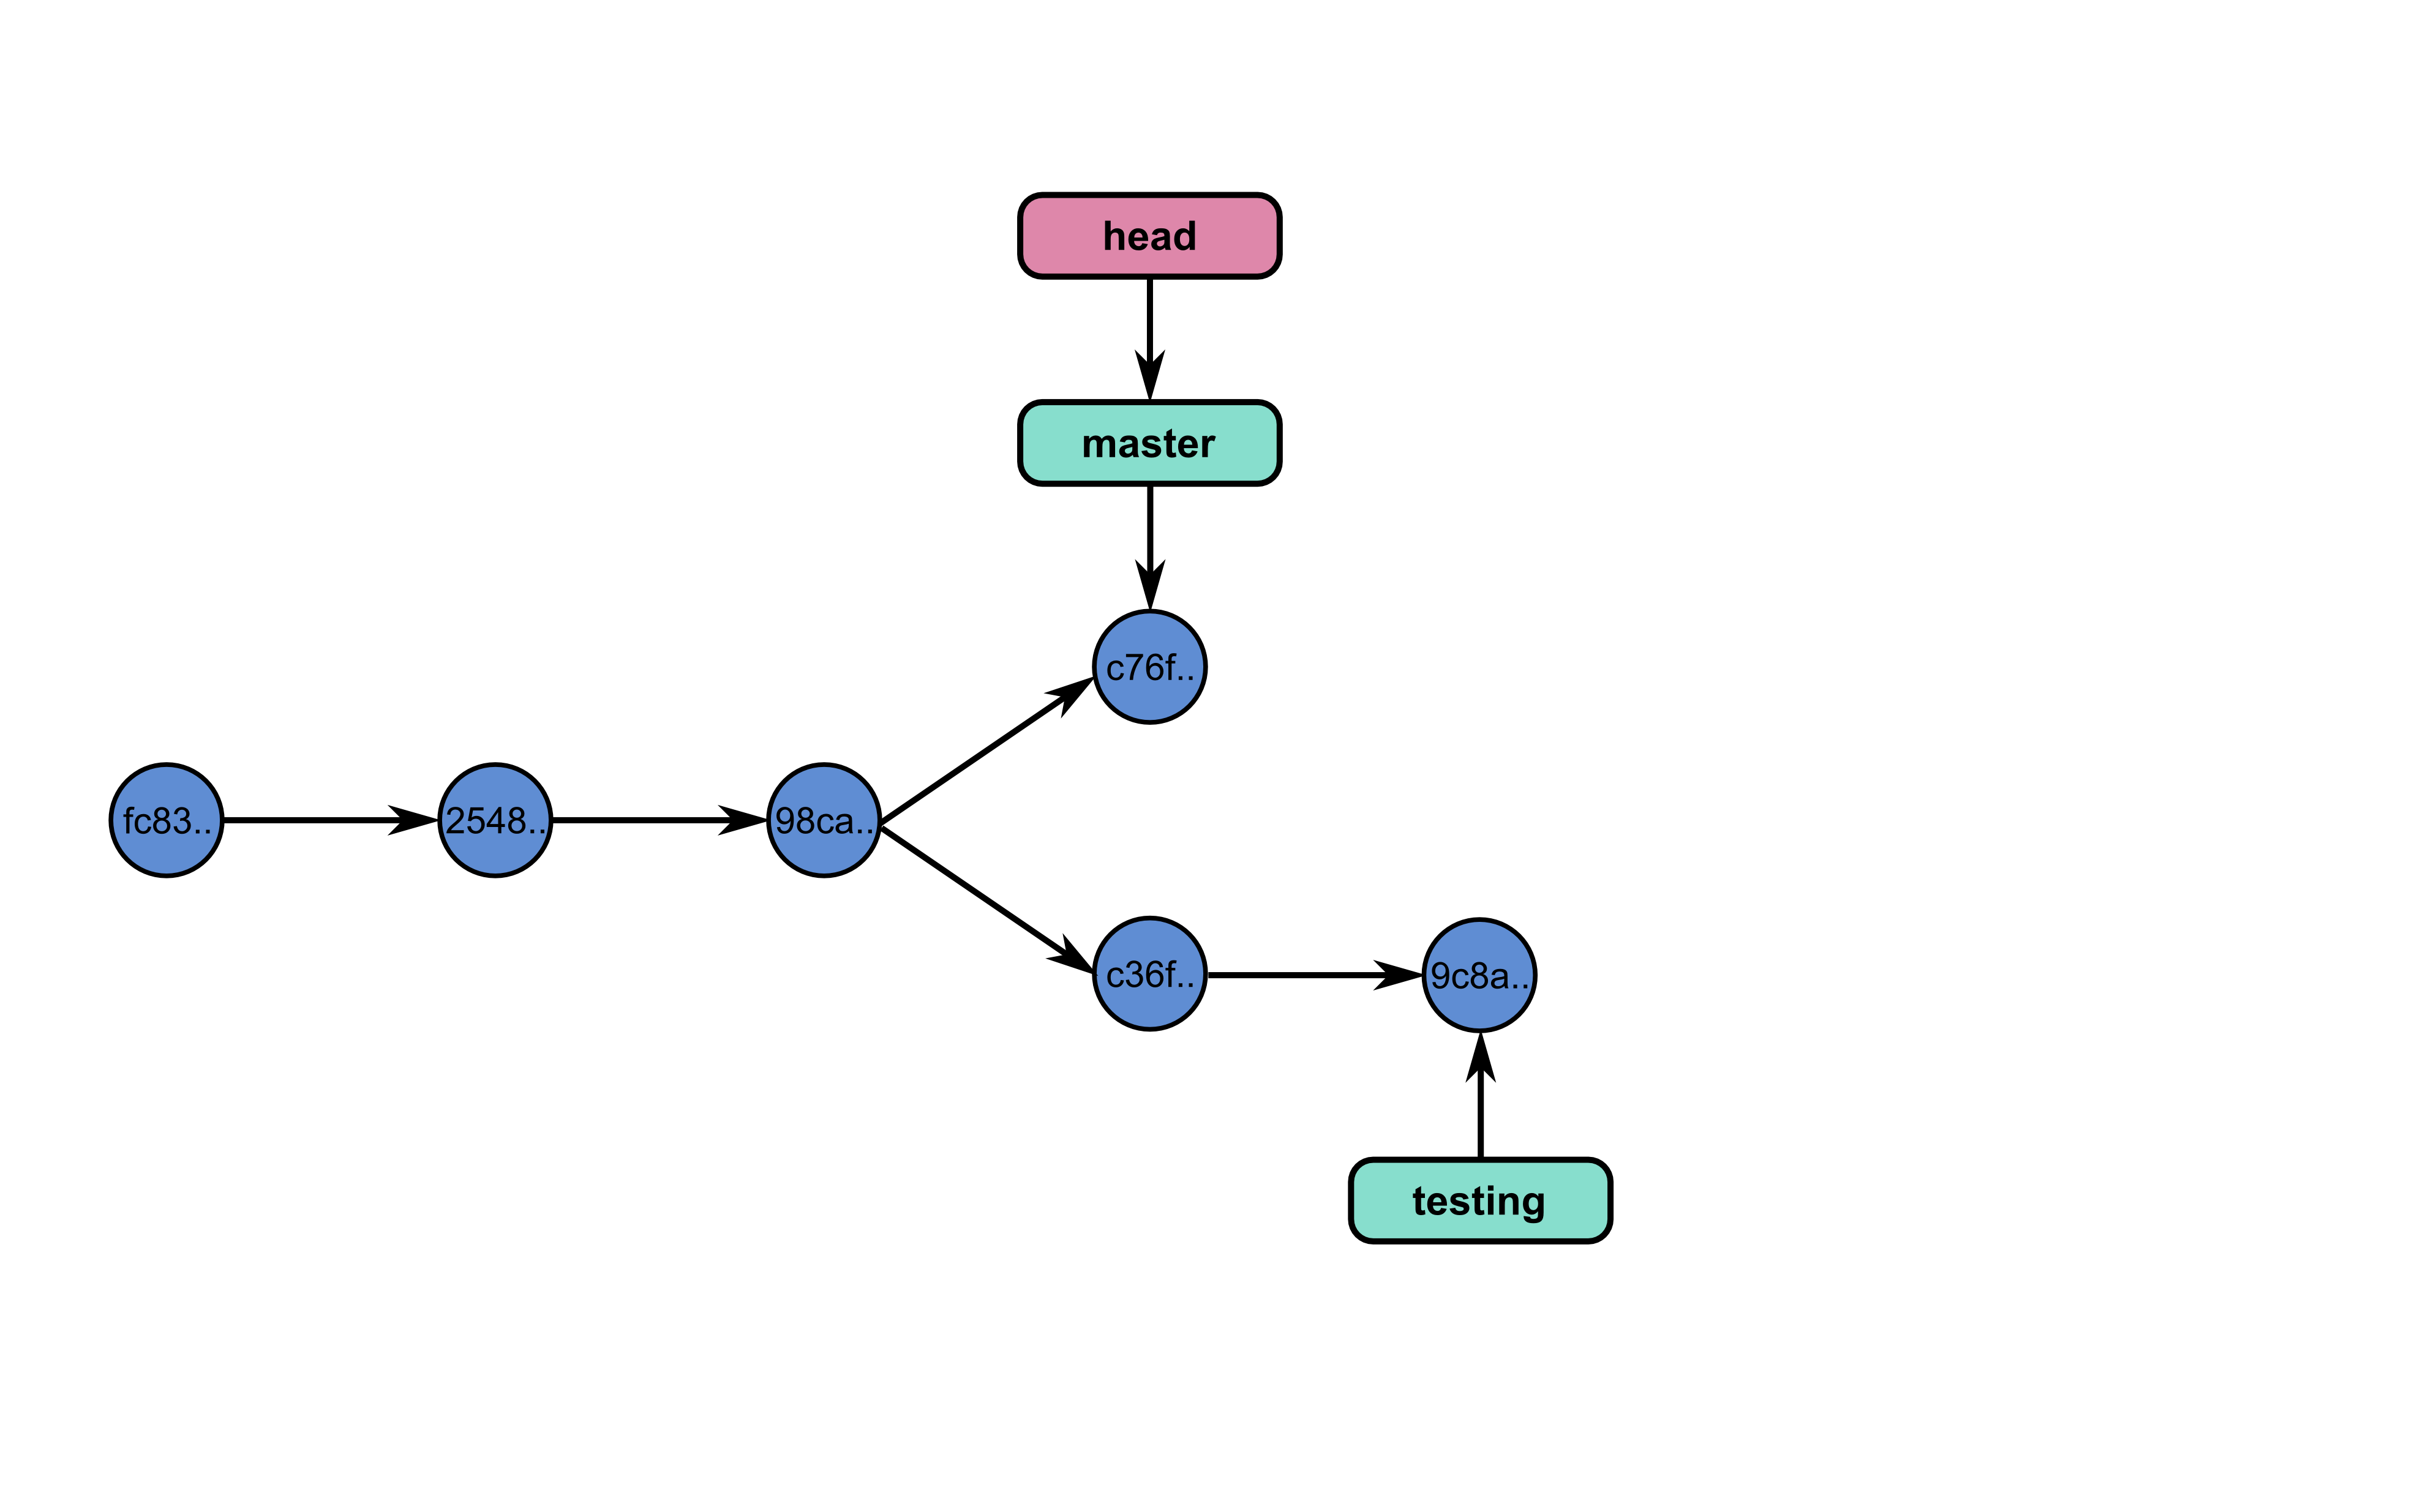
\includegraphics[scale=0.35]{branch4.png}
\end{figure}


\end{frame}

% --- Slide

\begin{frame}[fragile]
\frametitle{Merging}
Merge testing into master
\begin{figure}[htp]
 \centering
 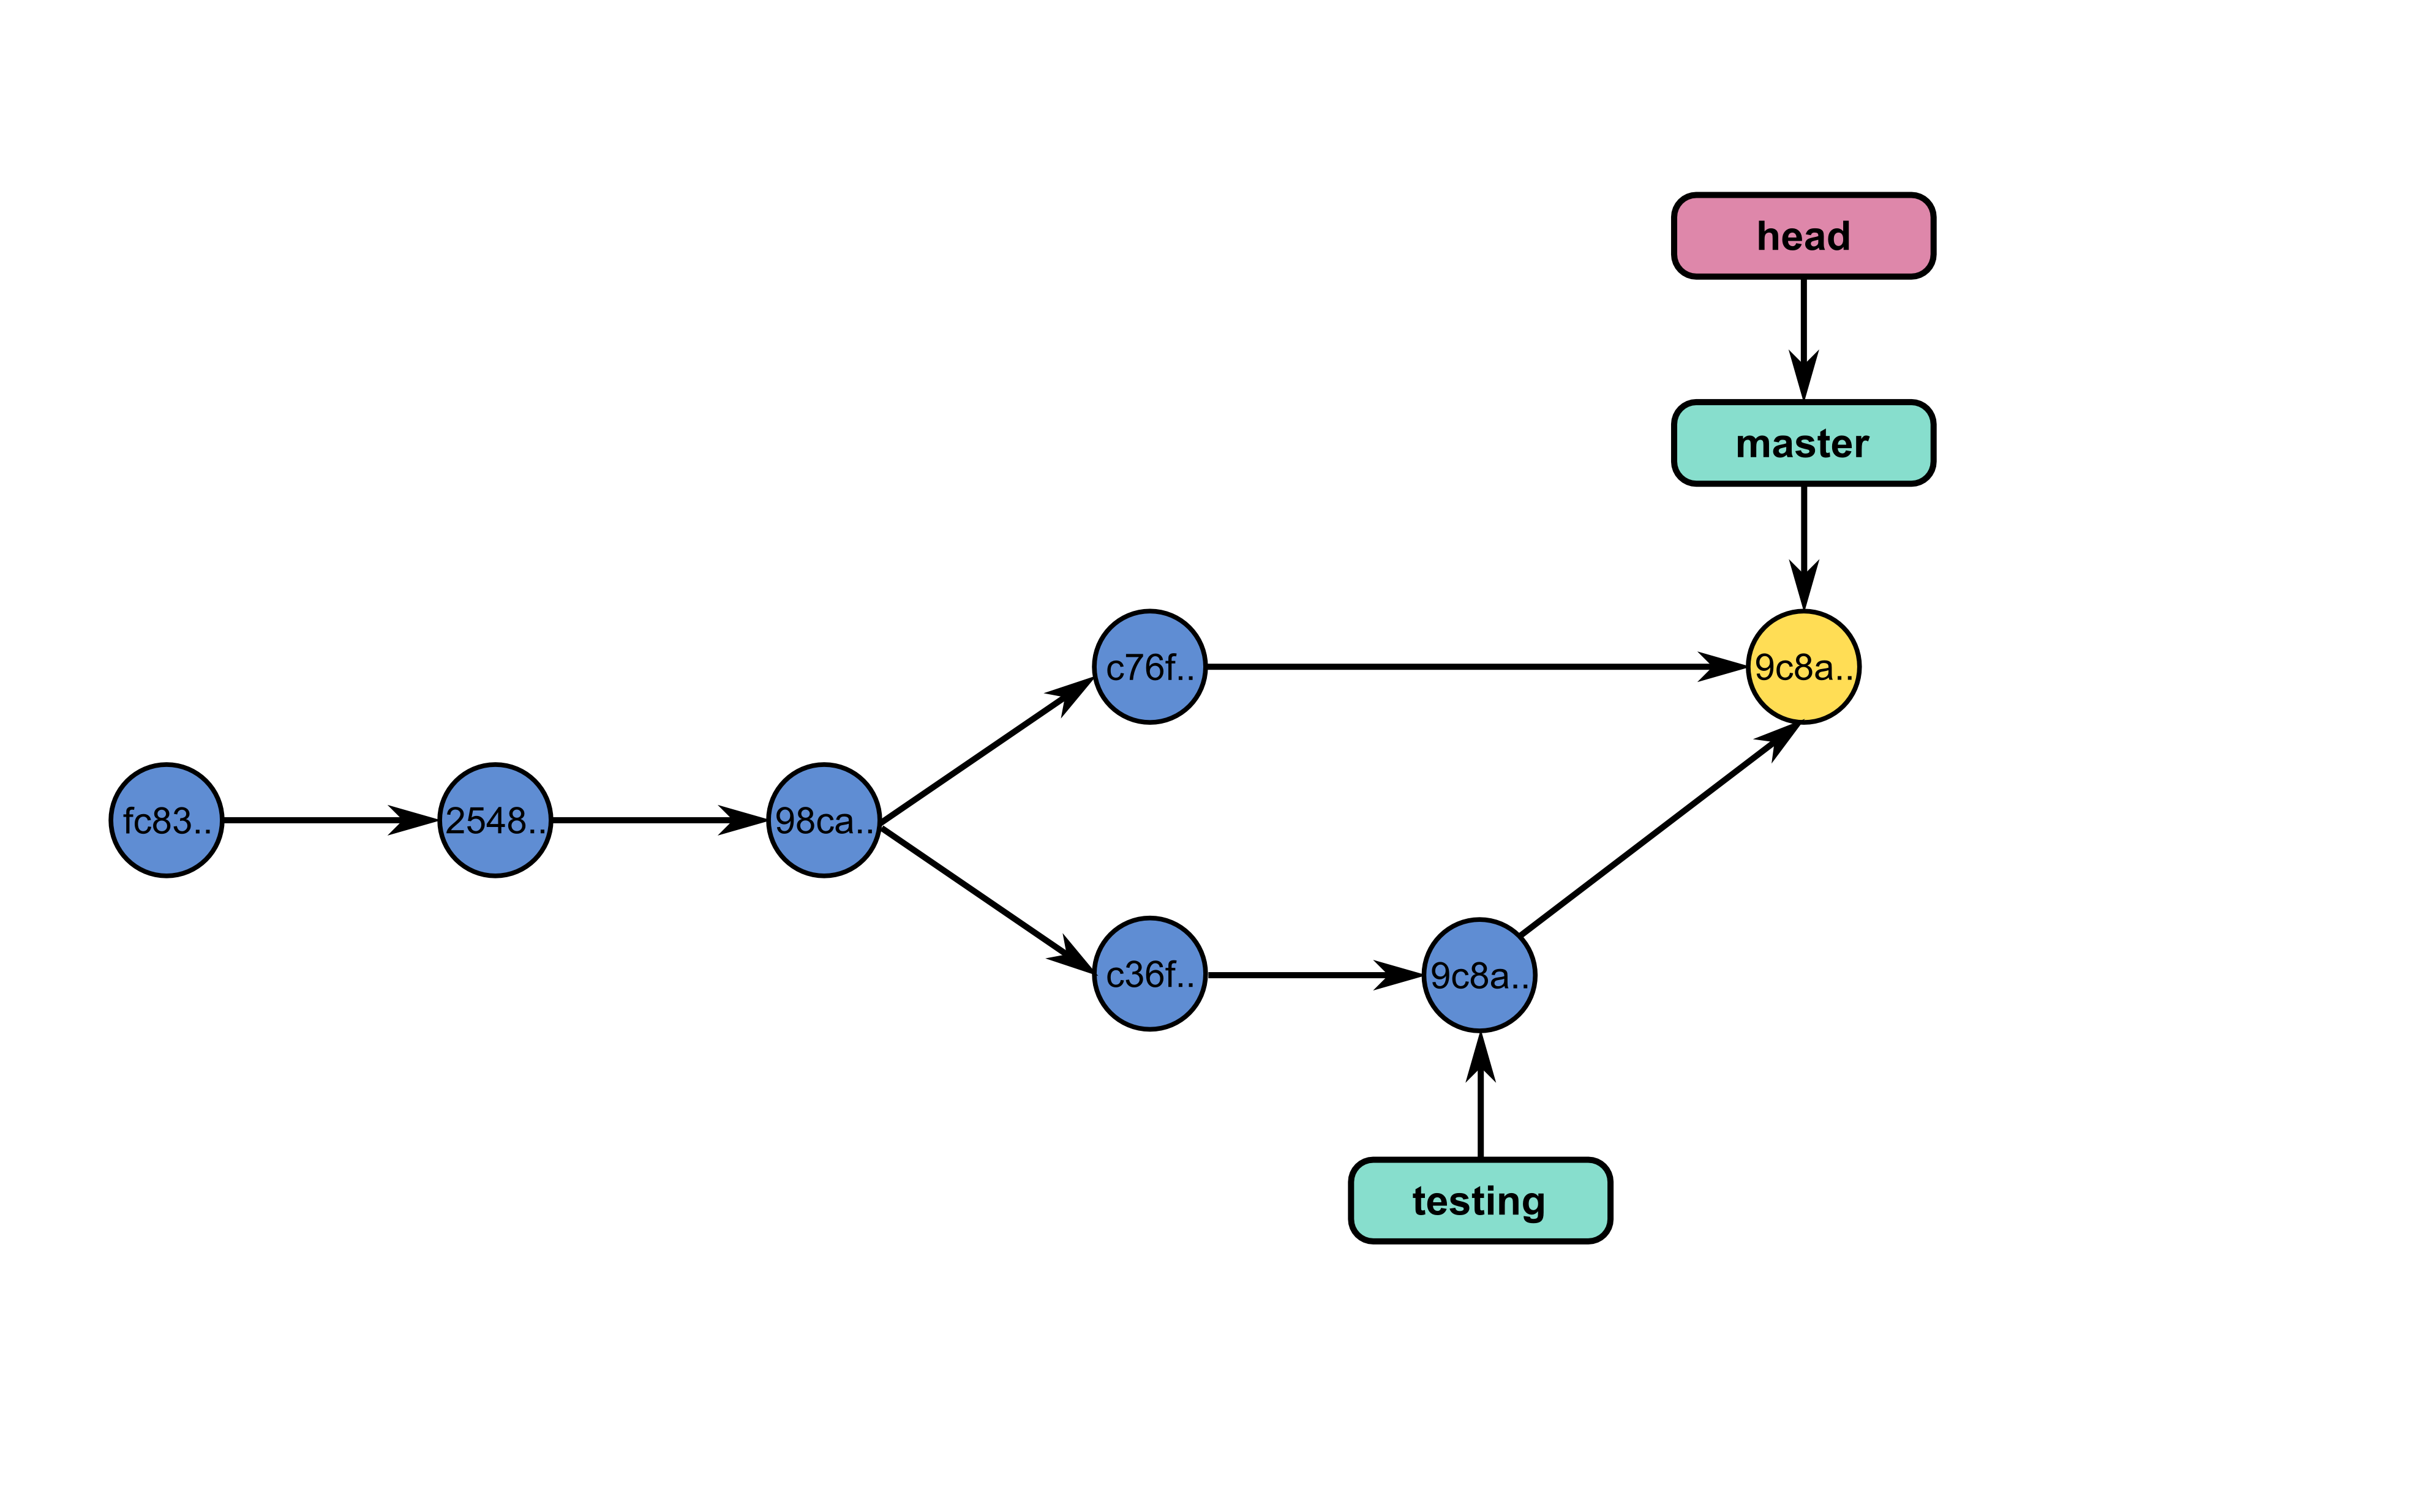
\includegraphics[scale=0.35]{branch5.png}
\end{figure}


\end{frame}

% --- Slide

\begin{frame}[fragile]
\frametitle{Merging}
\begin{figure}[htp]
 \centering
 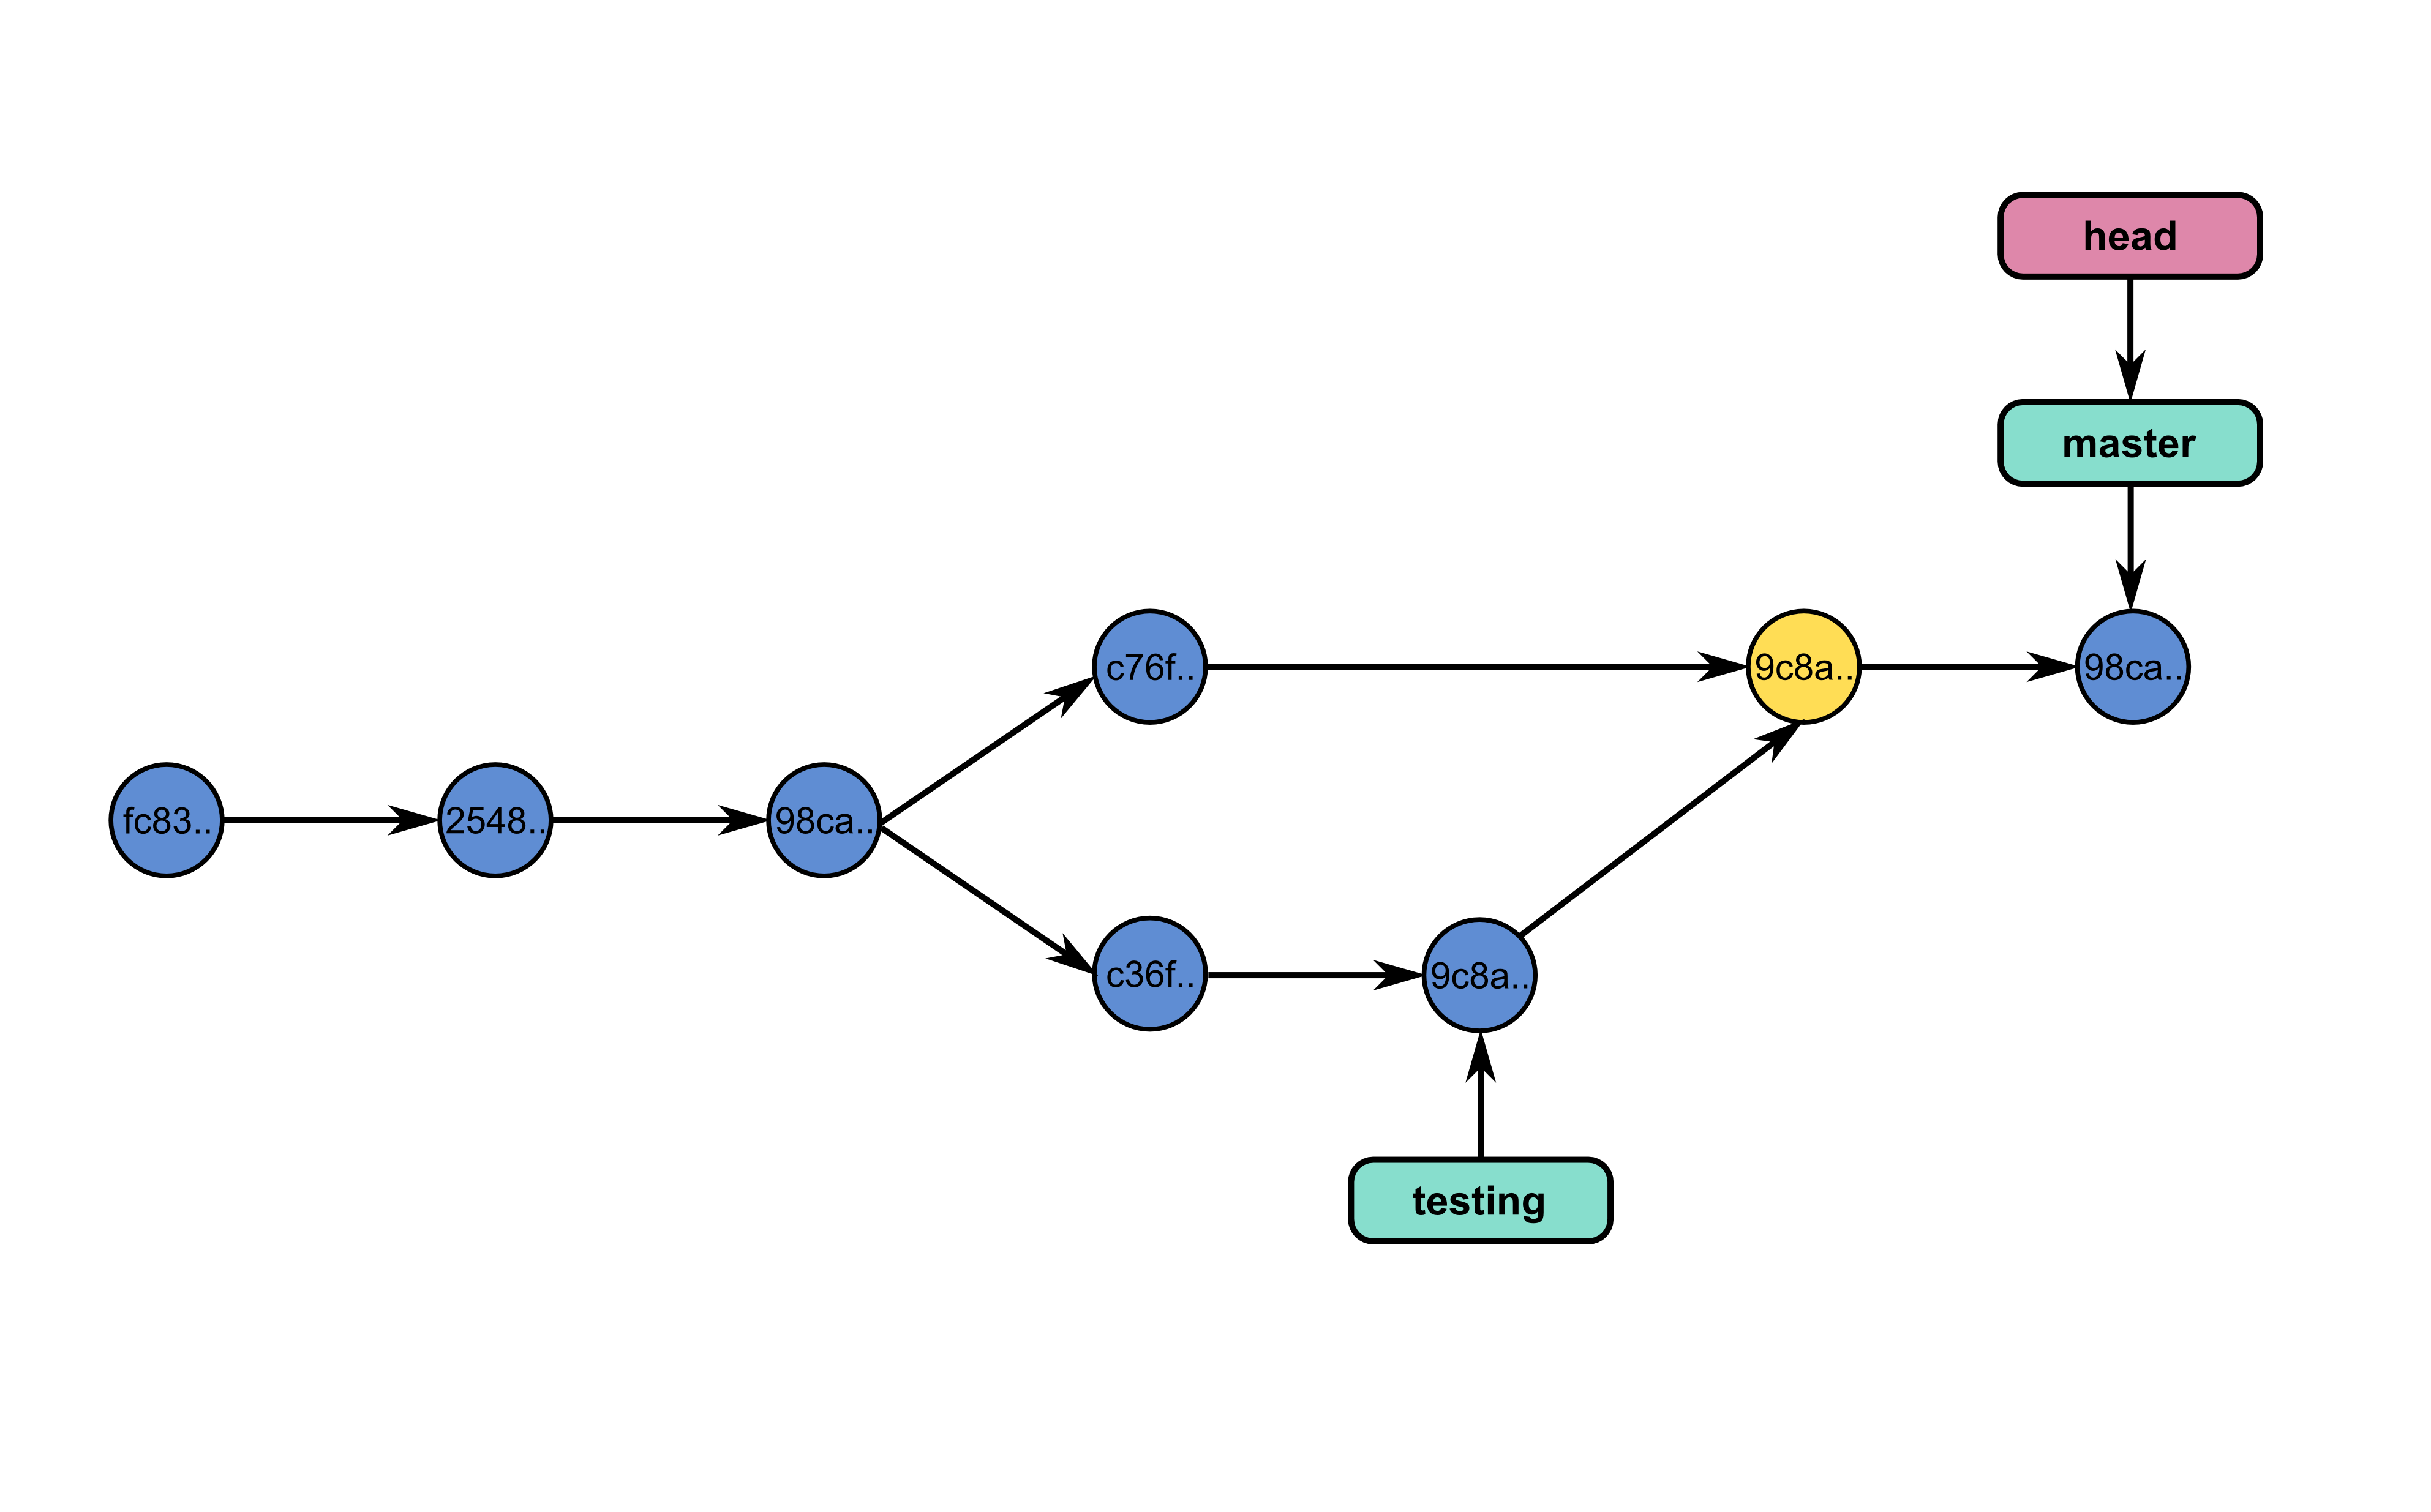
\includegraphics[scale=0.35]{branch6.png}
\end{figure}


\end{frame}



% --- Slide

\begin{frame}[fragile]
\frametitle{Remotes}

\begin{figure}[htp]
 \centering
 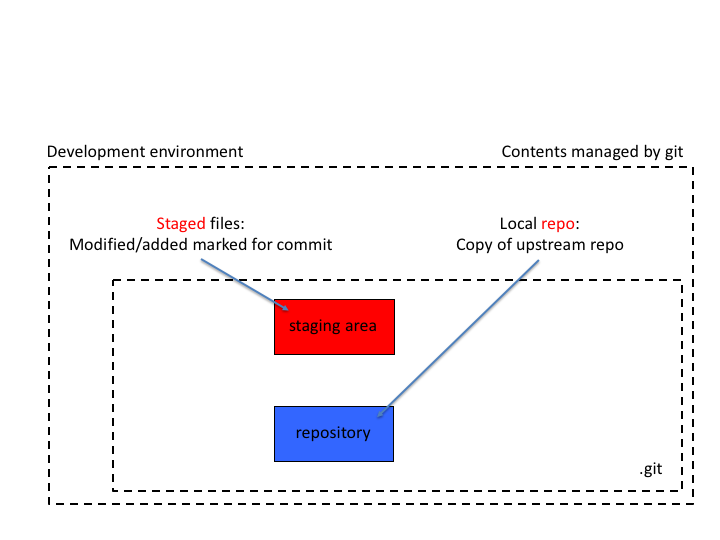
\includegraphics[scale=0.35]{gitC.png}
\end{figure}

\end{frame}

% --- Slide

\begin{frame}[fragile]
\frametitle{Remotes}

\begin{figure}[htp]
 \centering
 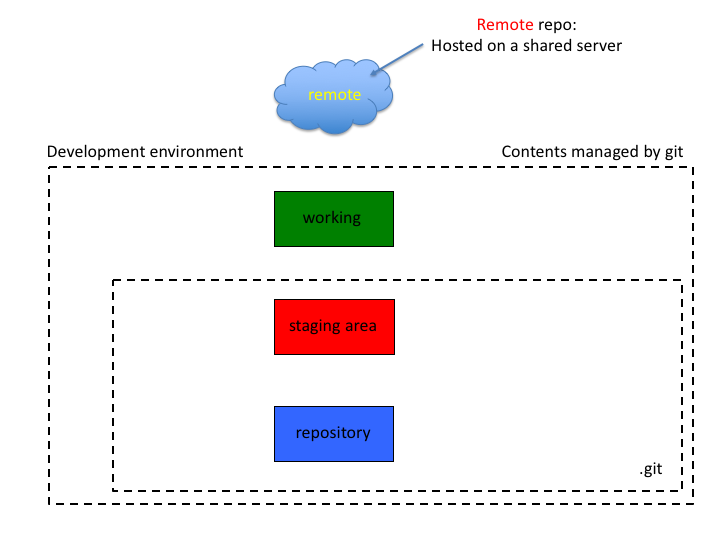
\includegraphics[scale=0.35]{gitD.png}
\end{figure}

\end{frame}


% --- Slide

\begin{frame}[fragile]
\frametitle{Git workflow}
\begin{figure}[htp]
 \centering
 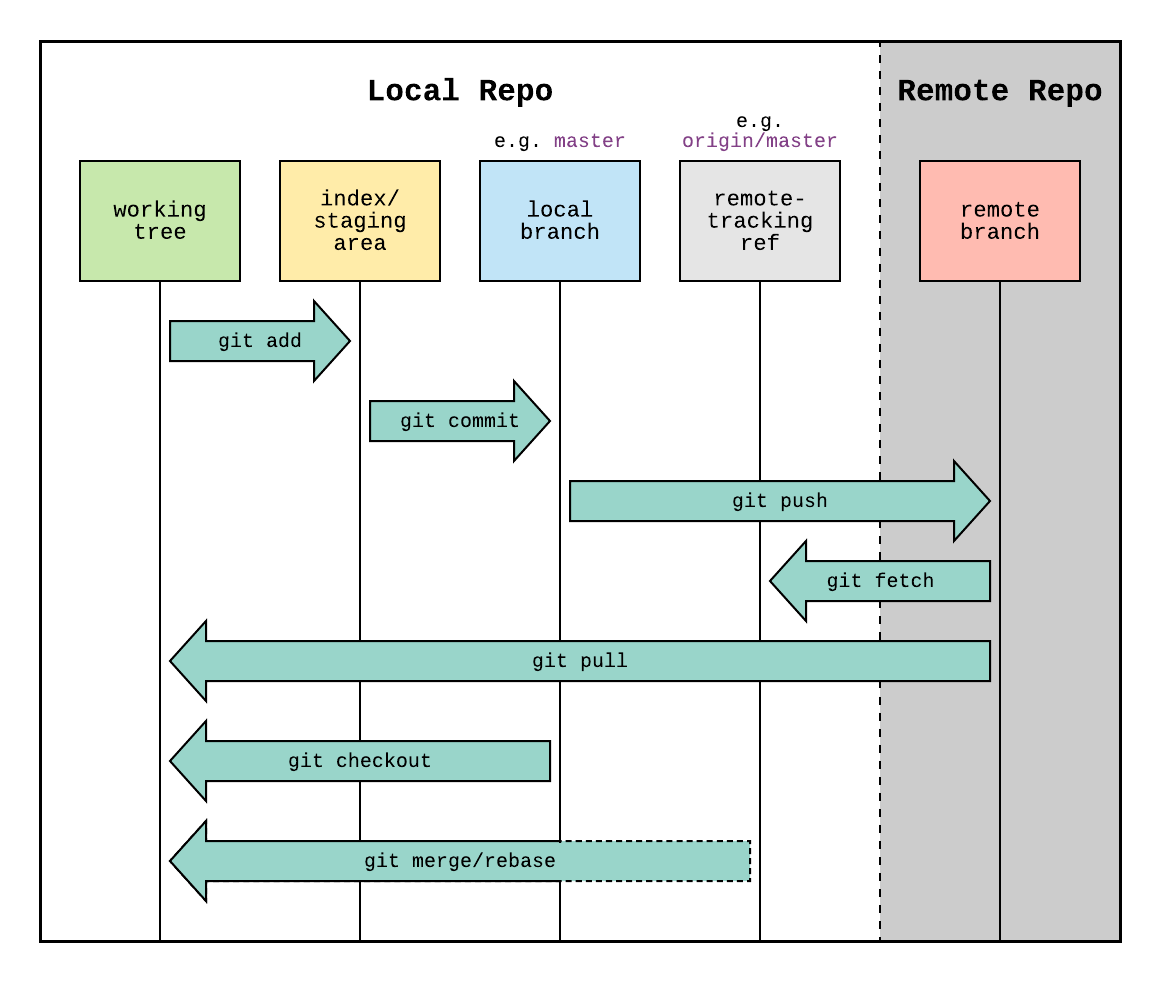
\includegraphics[scale=0.20]{gitWorkflow.png}
\end{figure}


\end{frame}


% --- Slide

\begin{frame}[fragile]
\frametitle{Resources}

\begin{itemize}
\item \href{http://book.git-scm.com/}{Git Community Book}
\item  \href{http://progit.org/book/}{Pro Git}
\item \href{http://marklodato.github.io/visual-git-guide/index-en.html}{A Visual Git Reference}
\item \textcolor{red}{\href{https://education.github.com/git-cheat-sheet-education.pdf}{Git Cheat Sheet}}
\end{itemize}


\end{frame}

\end{document}
